\documentclass[main.tex]{subfiles}

\begin{document}
\section{Preliminary Test and Motivation}
The motivation for this work was to understand, refine, and document the \disp method of direction reconstruction. This method was expected to be useful to better resolve objects observed close to the horizon and facilitate studying the stability of the reconstruction to the zenith angle of observation. There was also the possibility of using machine learning algorithms to improve resolution beyond that of the standard geometric reconstruction. In particular, an improved angular resolution on the Crab may open up the possibility of resolving the spatial extent of the Crab Nebula with the VERITAS instrument.

For the purposes of this work, the 68\% containment radius in angular position (\rse\hspace{-4pt}) is used as a measure of angular resolution and performance of the reconstruction. This was measured in two ways - one numerically and one using a 2D Gaussian fit of the 2D projection of the 3D deviation of the reconstruction. From here (see Fig. \ref{fig:sim_gauss}) it was clear that the Gaussian fit was not an accurate representation of the underlying data, but could nevertheless provide some insight into it.

\begin{figure}[H]
  \begin{center}
    \subfigure[A histogram of the 2D projection of the 3D angular deviation of the reconstructed direction. The colors denote the number of entries in a given bin.]{ 
      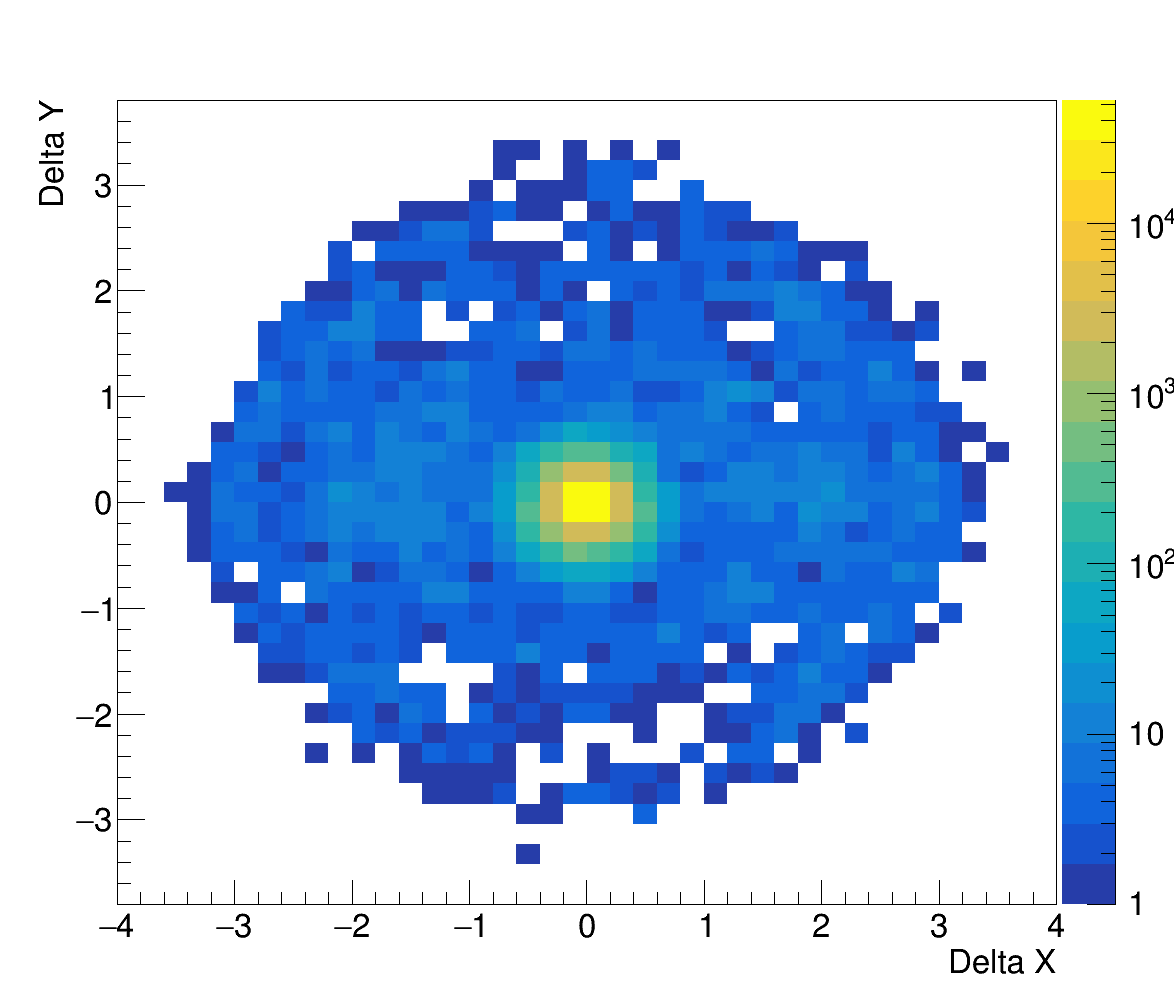
\includegraphics[width=0.44\linewidth]{sim_gauss_2D}
      \label{fig:sim_2D_gauss}
    }
    \hfill
    \subfigure[The radial deviation of the reconstructed direction for a diagonal slice of the 2D histogram where $\Delta Y\in \Delta X+(-0.05,0.05)$.]{ 
      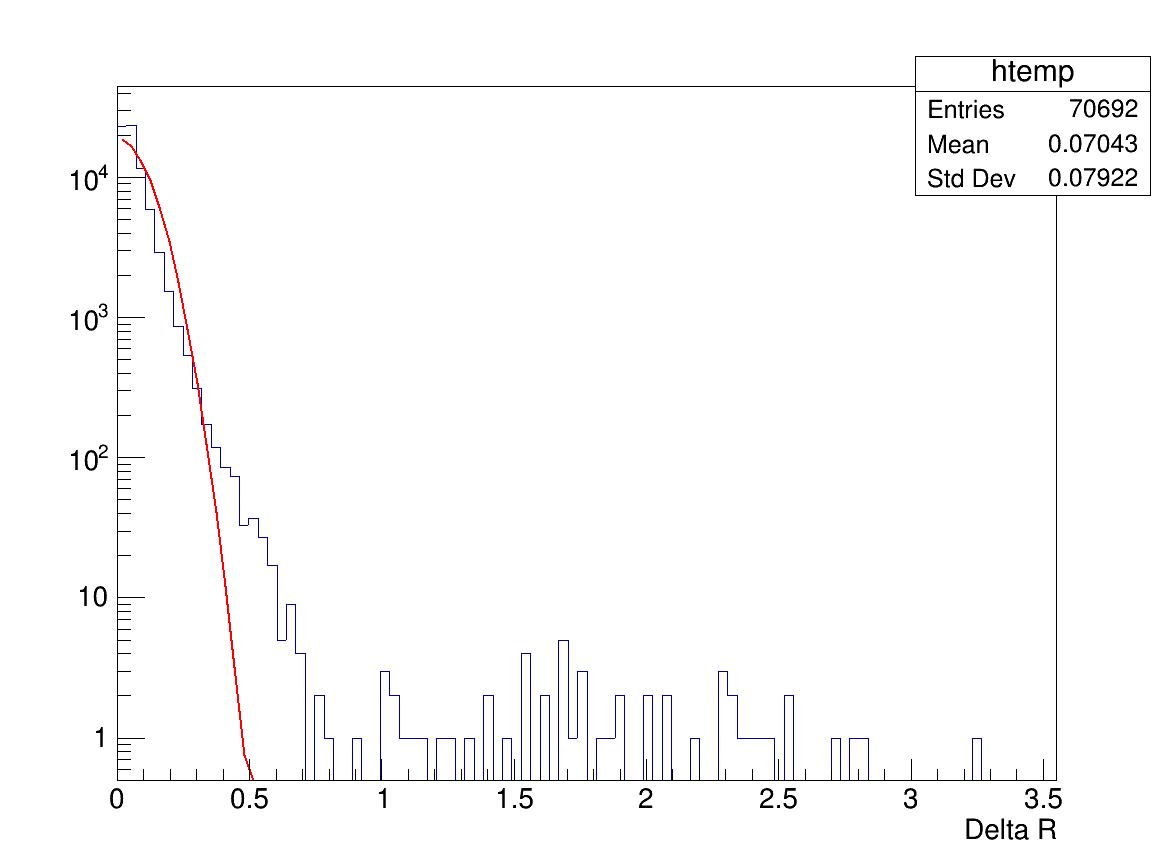
\includegraphics[width=0.44\linewidth]{radial_sim_gauss}
      \label{fig:sim_1D_radial_gauss}
    }
    \subfigure[The distribution (in $\Delta X$) of the reconstructed direction for a horizontal slice of the 2D histogram where $\Delta Y\in(0.0,0.2)$. There is a clear central Gaussian shape in the central $1^\circ$ region of the plot, in addition to a shorter, wider Gaussian with amplitude $\sim 10^{-3}$ times that of the central Gaussian.]{ 
      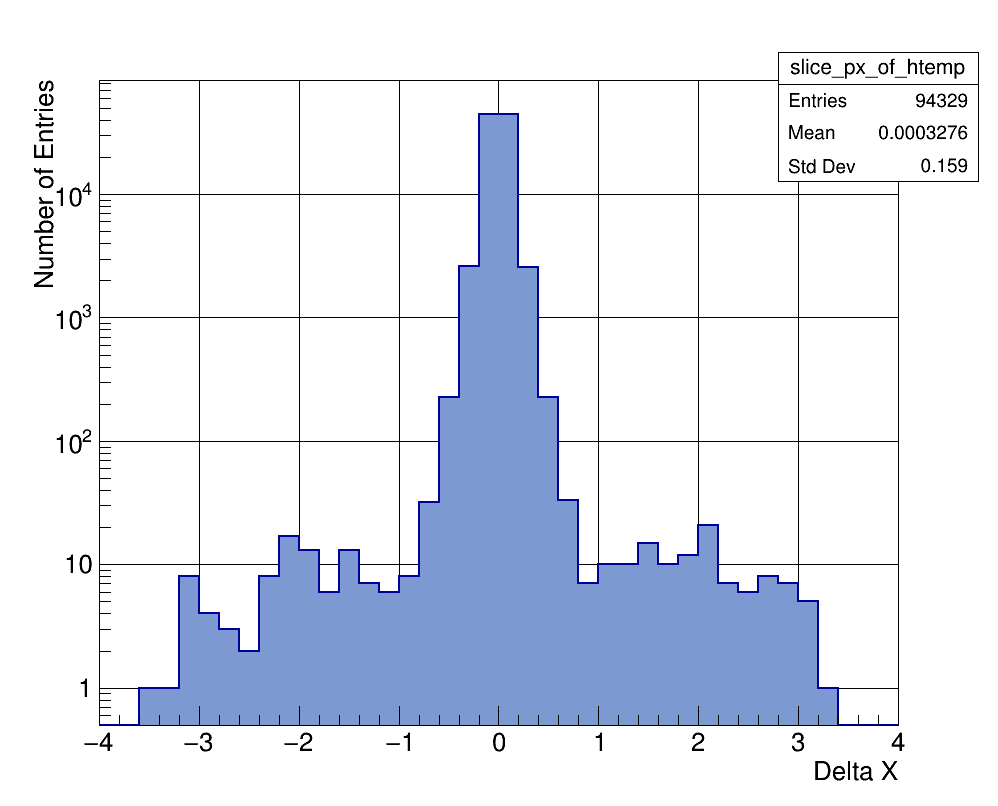
\includegraphics[width=0.44\linewidth]{slice_sim_gauss1}
      \label{fig:sim_1D_gauss1}
    }
    \hfill
    \subfigure[The distribution (in $\Delta X$) of the reconstructed direction for a horizontal slice of the 2D histogram where $\Delta Y\in(0.8,1.0)$.]{ 
      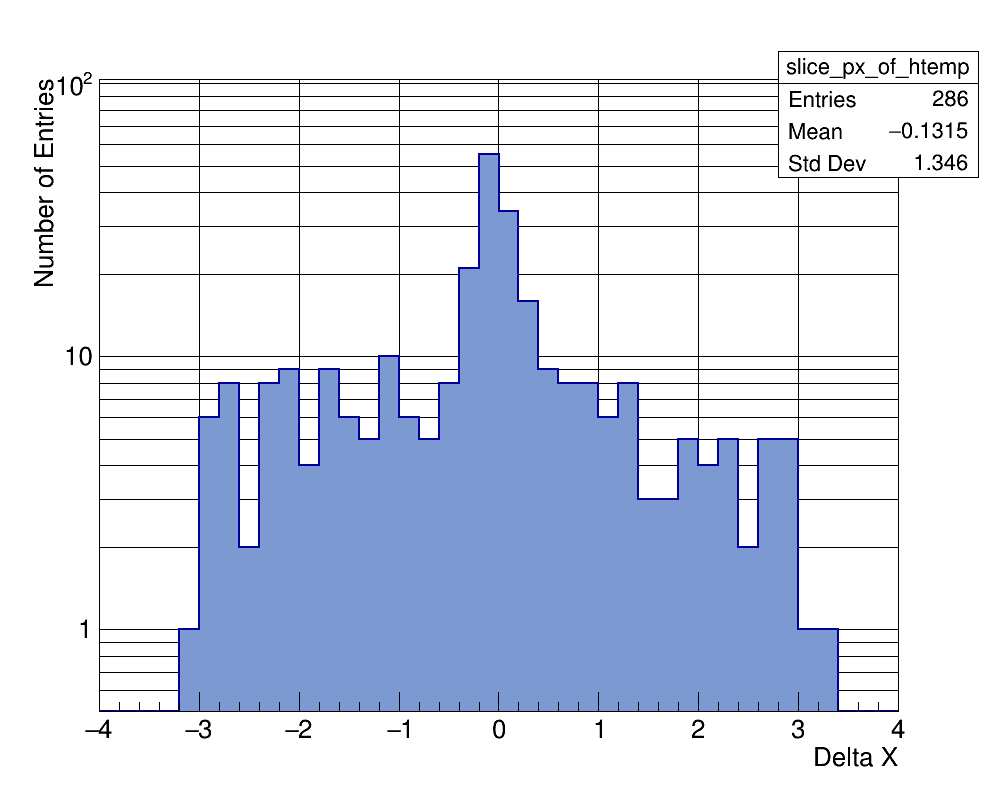
\includegraphics[width=0.44\linewidth]{slice_sim_gauss2}
      \label{fig:sim_1D_gauss2}
    }
  \end{center}
  \caption[Gaussian shape of the simulation deviation.]{Reconstruction of the simulation direction using the \disp Method for simulations at $45^\circ$ zenith angle with $10^{3}$ GeV$<E<10^{3.5}$ GeV. From here it is evident that a \rse based on the width of the best-fit Gaussian would not be an accurate measure of the \rse, and would consistently overestimate the resolving power of the method. However, it is also clear that the vast majority of statistics fall in the central region, and that the width of this region can provide a first-order approximation to the R$_{68}$.}
  \label{fig:sim_gauss}
\end{figure}

Based on the distribution of the deviation of reconstructed direction of the simulations (Fig. \ref{fig:sim_gauss}) from the simulated direction, it was determined that a fit to the central Gaussian could provide some useful information about the R$_{68}$, and to this end, the 2D distribution (Fig. \ref{fig:sim_2D_gauss}) was fit with the superposition of two Gaussians, with the68\% of this superposition as a first-order approximation to the R$_{68}$. Additionally, it was determined a numerical integral would provide a more accurate measure of this quantity and so the distribution of radial deviations was integrated from the tail inwards, until 32\% of the events were counted and this value of the radial deviation from the simulated direction was used as a more accurate measure of the R$_{68}$, a representative sample of the results is shown in Fig. \ref{fig:gauss_fit_both}.
\begin{figure}[htbp]
  \centering
  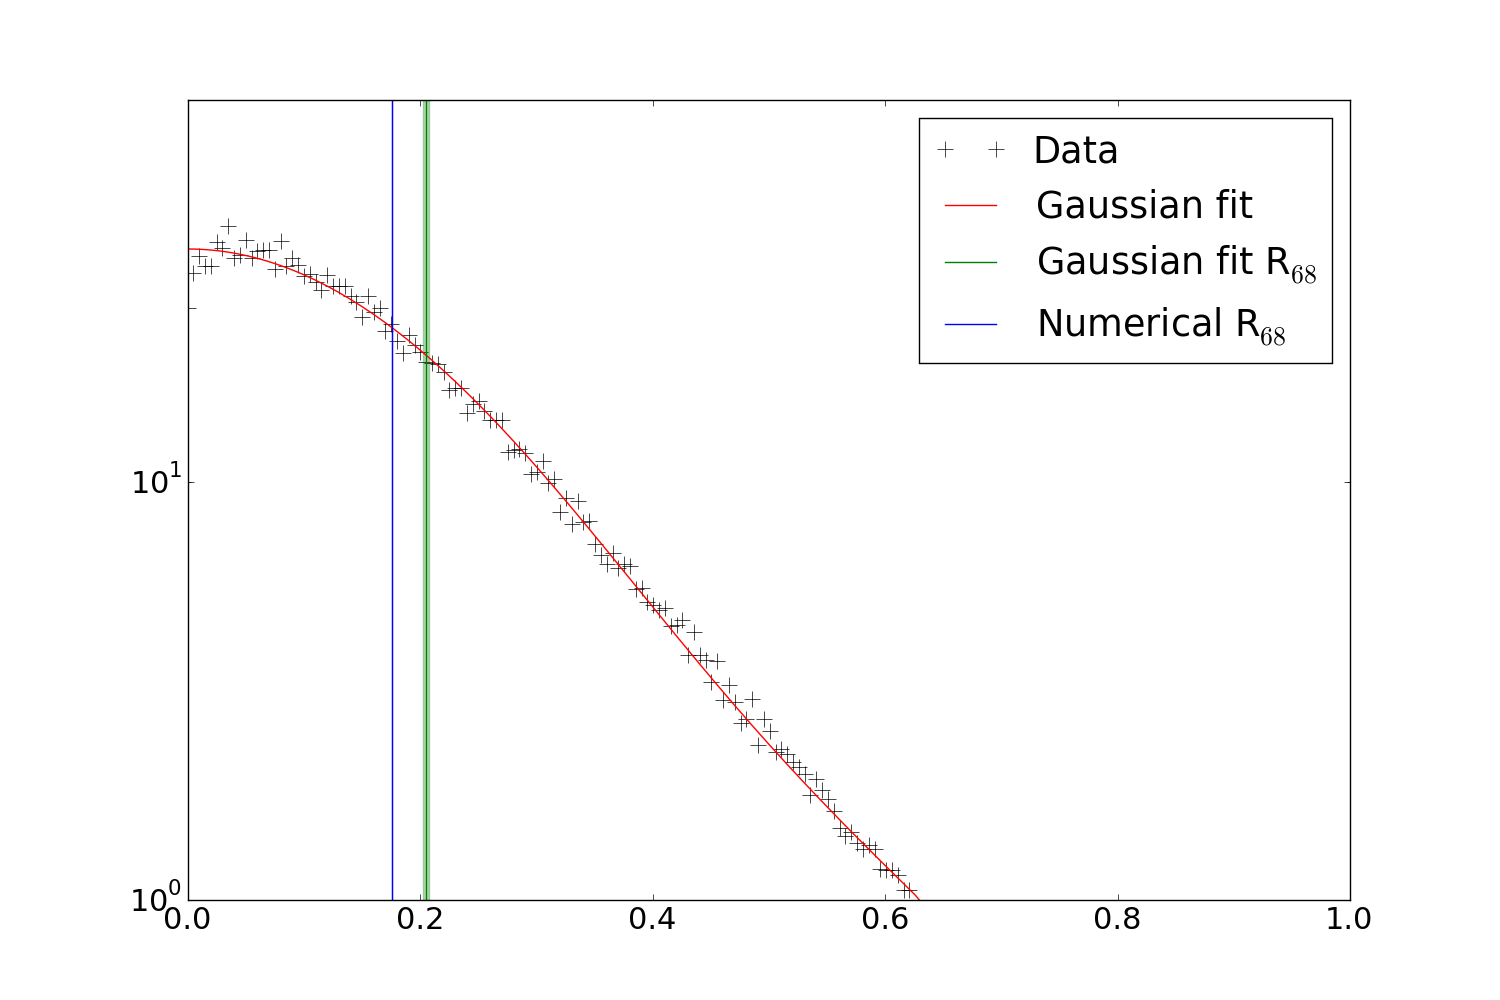
\includegraphics[width=.78\linewidth]{fit/gauss_fit_both}
  \caption[\rse from the Gaussian fit and the numerical integral.]{The \rse calculated for a simulation using a fit to a superposition of two Gaussians (green vertical line) and a numerical integration from $1^\circ$ inwards (blue vertical line), overlaid on a radial slice for Monte-Carlo simulations.}
  \label{fig:gauss_fit_both}
\end{figure}

A preliminary test for the \rse of the data was enabled by a set of runs where the Crab was tracked from horizon to culmination and back to the horizon (from the nights of Jan 12 2018, Jan 13 2018, and Jan 04, 2019). This provided a reference data set with high significance to track the energy and zenith dependences of the direction reconstruction in stable (and therefore directly comparable) weather conditions. The differential resolution for the Crab data was measured in several energy and zenith bins and is presented in Fig. \ref{fig:crab_initial}.

\begin{figure}[H]
  \begin{center}
    \subfigure[Crab reconstructed resolution using Method0.]{ 
      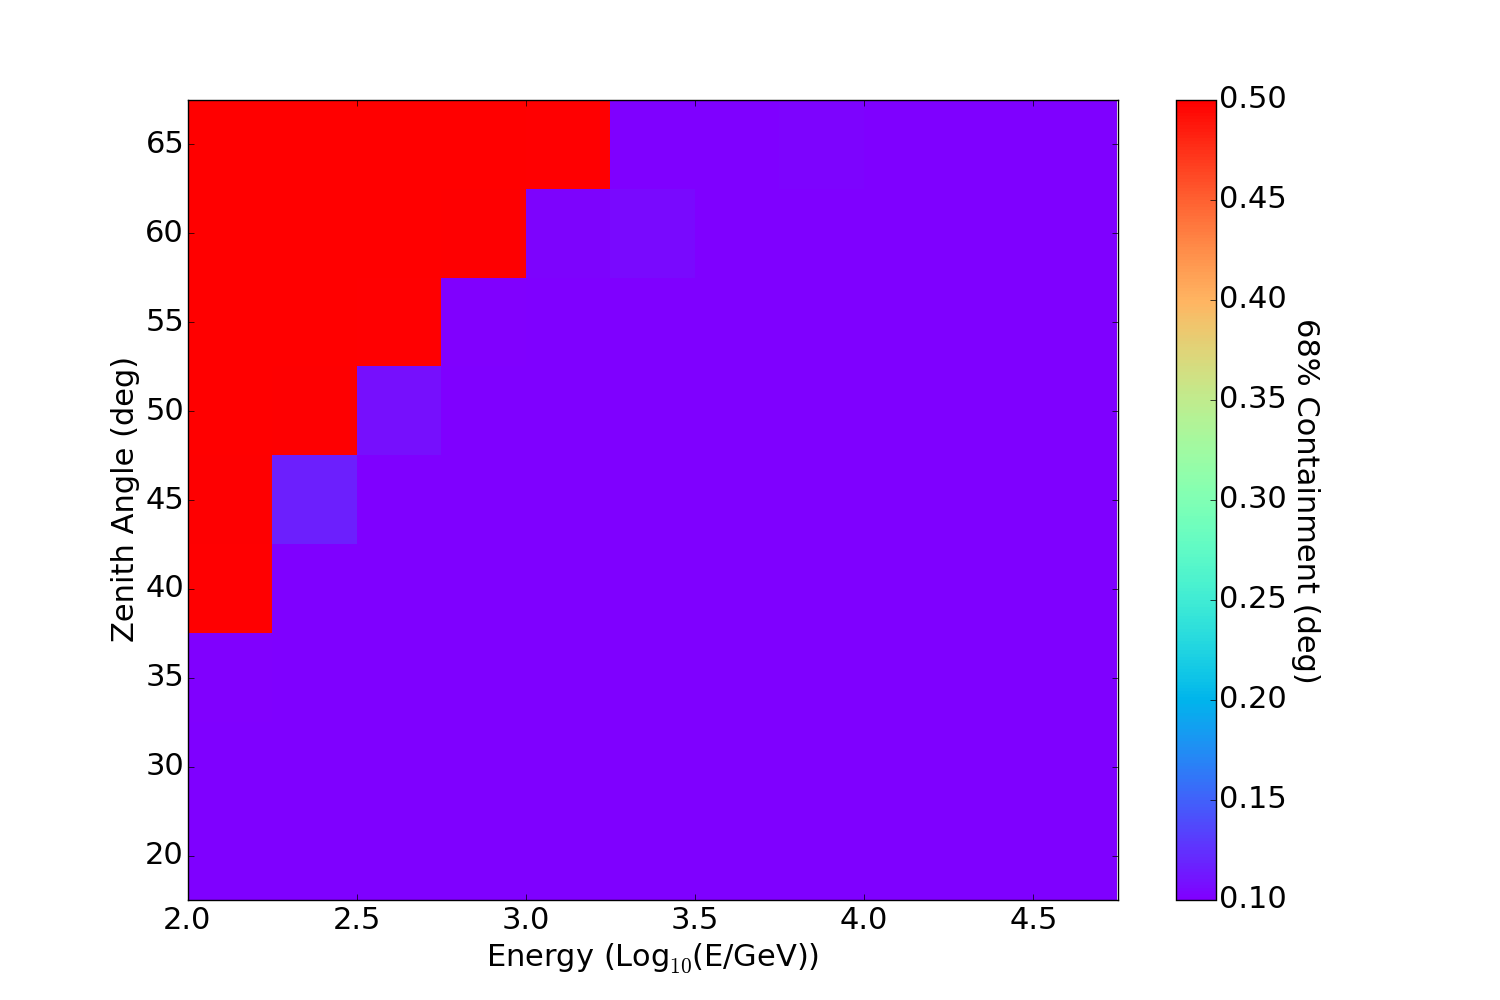
\includegraphics[width=0.47\linewidth]{num/LZA_data_25/crab_reg_rse.png}
      \label{fig:crab_reg_res}
    }  
    \subfigure[Crab binned significance.]{ 
      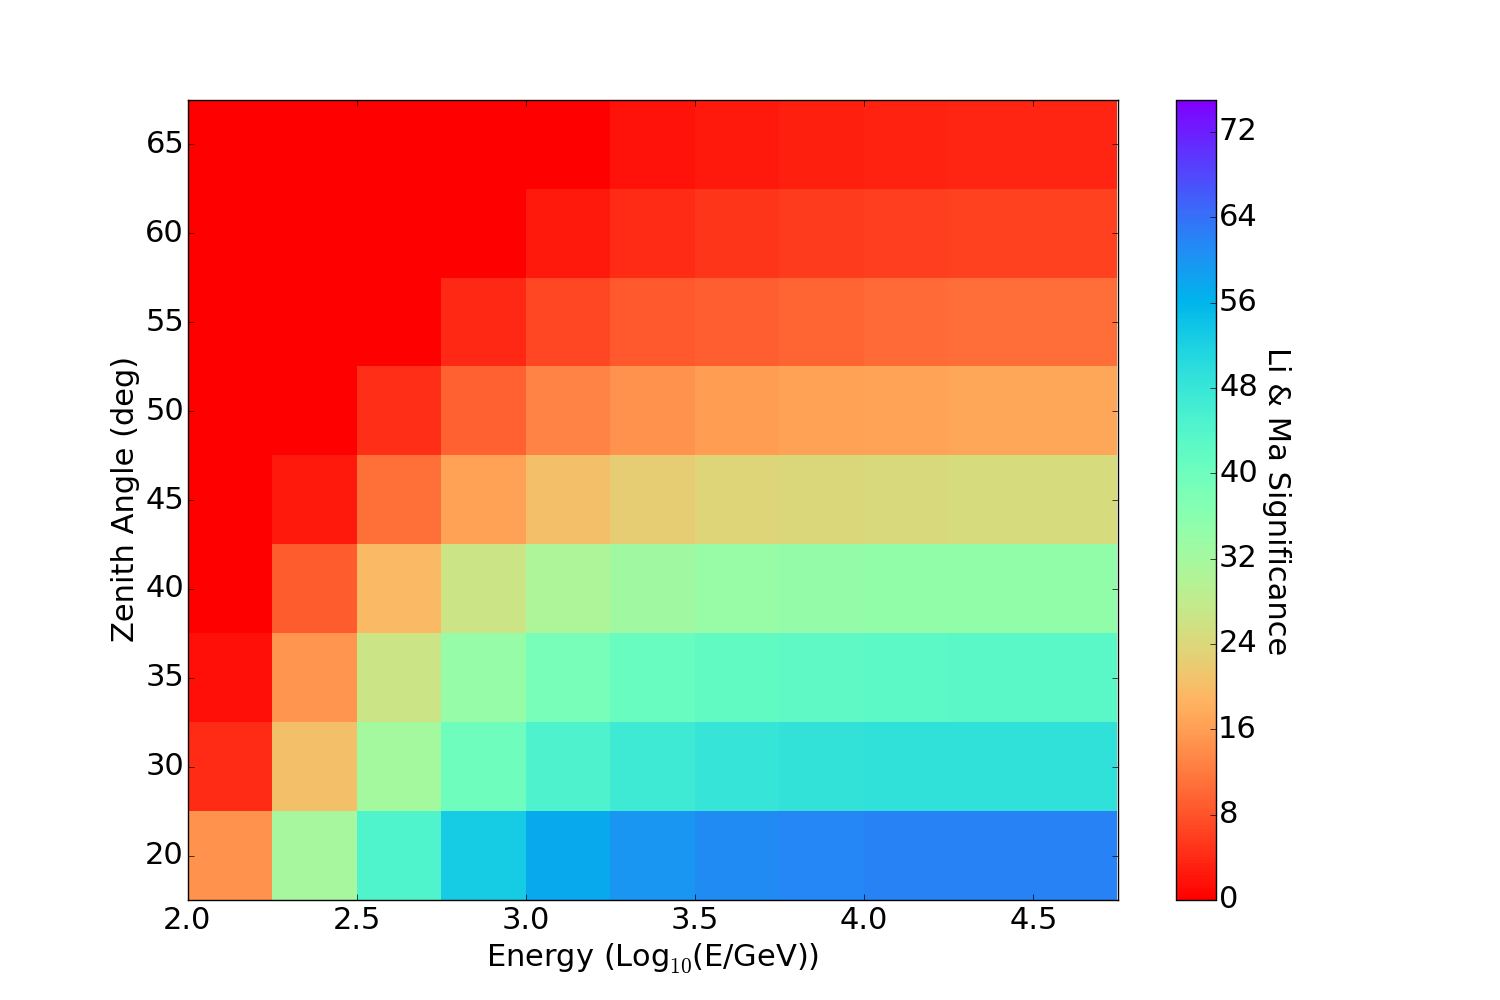
\includegraphics[width=0.47\linewidth]{num/LZA_data_25/crab_reg_LiMa.png}
      \label{fig:crab_res_num}
    }
  \end{center}
  \caption[Crab direction reconstruction using Method0.]{Reconstruction of the Crab direction using Method0 (standard geometric reconstruction from \textit{VEGAS}). On the left, the regions of white denote regions where significance $<3\sigma$.}
  \label{fig:crab_initial}
\end{figure}



\section{\disp Table and \rse Dependencies}
The BDT weight tables were generated independently of the old \disp method in order to have well-understood documentation of the underlying effects and dependencies.

\subsection{Zenith Angle Dependence}
A set of \disp tables was generated with a small sample of simulated events ($n\approx 1.9\e6$) across the range of zenith angles of interest ($20^\circ-65^\circ$). This was compared to the regular \disp method. Since there was no record of the training sample size for the standard tables, this test sample was useful in determining the resolution of the \disp method with a relatively small computational footprint. Additionally, it allowed for some simple tests of dependence of the \disp tables on parameters not explicitly in the \disp tables.

These small \disp tables and the standard \disp tables were used to reconstruct simulation events and compared with Method0 (the standard method of direction reconstruction). In both cases, the \disp method performs better than Method0 at the largest zenith angles ($\geq 55^\circ$, see \ref{fig:olddisp_ratio}-\ref{fig:disp_ratio_250} for \rse of the \disp methods divided by that for Method0 at the same zenith angle).

\begin{figure}[H]
  \begin{center}
    \subfigure[Numerically determined R$_{68}$.]{
      \includegraphics[width=0.8\linewidth]{num/disp_standard_ratio_xzen}
      \label{fig:olddisp_ratio_num}
    }
    \subfigure[R$_{68}$ as determined from a fit.]{
      \includegraphics[width=0.8\linewidth]{fit/disp_standard_ratio_xzen}
      \label{fig:olddisp_ratio_fit}
    }
      \caption[``standard'' \disp table reconstruction.]{Ratio of \rse of the ``standard'' \disp table to that from Method0, with the numerically determined \rse (left) and that found from the fit to two Gaussians. Since this is the ratio of methods, the horizontal blue line denotes the performance using Method0; and the \disp method definitively performs better than Method0 for zenith $\gtrsim50^\circ$.}  
      \label{fig:olddisp_ratio}
  \end{center}
\end{figure}

From Fig. \ref{fig:olddisp_ratio}, we can see that the \disp method outperforms the standard method across zenith angles when using the numerical integration, i.e. the tails of the distribution from the geometric method are better behaved than those found using the \disp method. However, when using the fit which provides an understanding of the central region where most events lie, the \disp method outperforms the geometric reconstruction only in the LZA range ($\phi\gtrsim 50$). This is considered the regime of interest for the \disp method.

\begin{figure}[H]
  \centering
    \subfigure[Numerically determined R$_{68}$.]{
      \includegraphics[width=0.8\linewidth]{num/disp_250_ratio_xzen}
      \label{fig:disp_ratio_250_num}
    }
    \subfigure[R$_{68}$ as determined from a fit.]{
      \includegraphics[width=0.8\linewidth]{fit/disp_250_ratio_xzen}
      \label{fig:disp_ratio_250_fit}
    }
  \caption[Small \disp table reconstruction (noise = $250$ MHz).]{Ratio of the \rse from reconstruction using the small \disp table ($\sim 1.9\e6$ events all at noise $= 250$ MHz) and that from Method0 with the numerically determined \rse (left) and that found from the fit to two Gaussians. Note the horizontal blue line denotes the performance using Method0, so this method performs better than Method0 for zenith $\gtrsim 50^\circ$.}
  \label{fig:disp_ratio_250}
\end{figure}

\subsection{Over-training}
BDT-based regression is quite robust under non-linear correlations between discriminating parameters. The primary vulnerability of this method is that  to over-training - where the decision tree starts to be informed by noise and nuisance parameters in the training sample rather than relevant effects. This results in substantially different reconstruction efficiencies between training and testing samples. The ROOT TMVA package includes a test for over-training where it randomly selects a given fraction of the supplied events (for the purposes of this work, this fraction was taken to be 50\%) to use for testing. These events are then not used to train the regression trees and are instead used only to generate a measure of the over-training.
This check of the over-training for one of the test tables (noise $= 450$ MHz), shown in Fig. \ref{fig:overtraining}, demonstrates that there was no meaningful over-training of the table, at least based on effects present only in the training sample.

There remains however, the possibility of effects related to noise level that might appear in the training \textit{and} testing samples (which are generated separately at each noise level), but not in observational data sets, which would be overlooked by this measure of over-training.

\begin{figure}[H]
  \centering
  \subfigure[Deviation of reconstructed \disp parameter from Monte-Carlo \disp parameter in training sample.]{
    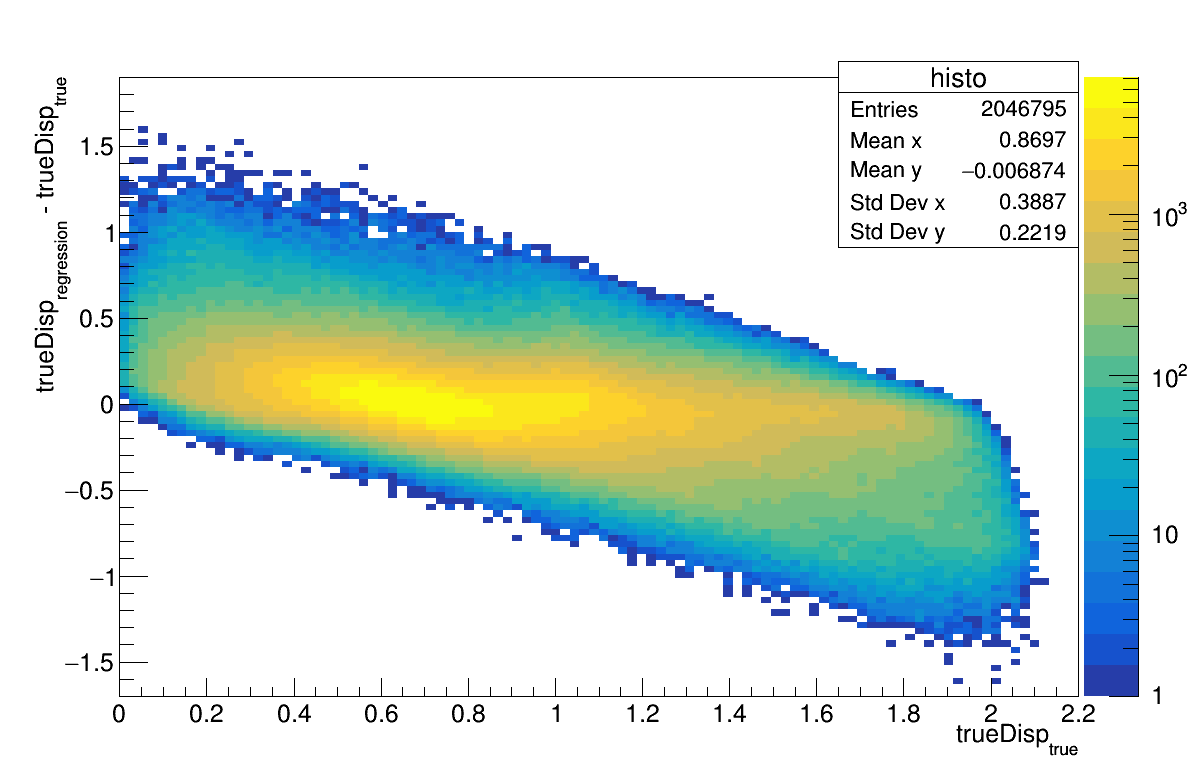
\includegraphics[width=.47\linewidth]{trueDisp_Train}
    \label{fig:disp_train_overtraining}
  }
  \subfigure[Deviation of reconstructed \disp parameter from Monte-Carlo \disp parameter in testing sample.]{
    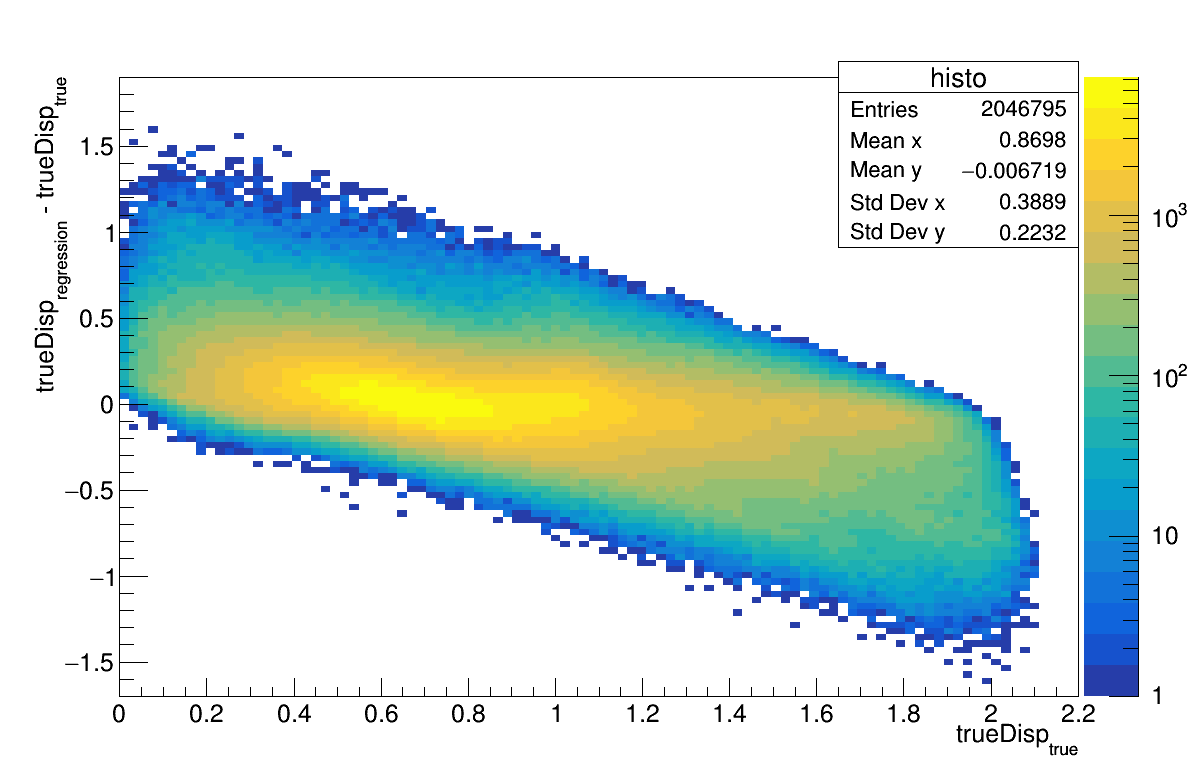
\includegraphics[width=.47\linewidth]{trueDisp_Test}
    \label{fig:disp_test_overtraining}
  }
  \subfigure[Deviation of reconstructed \disp Error parameter from Monte-Carlo \disp Error parameter in training sample.]{
    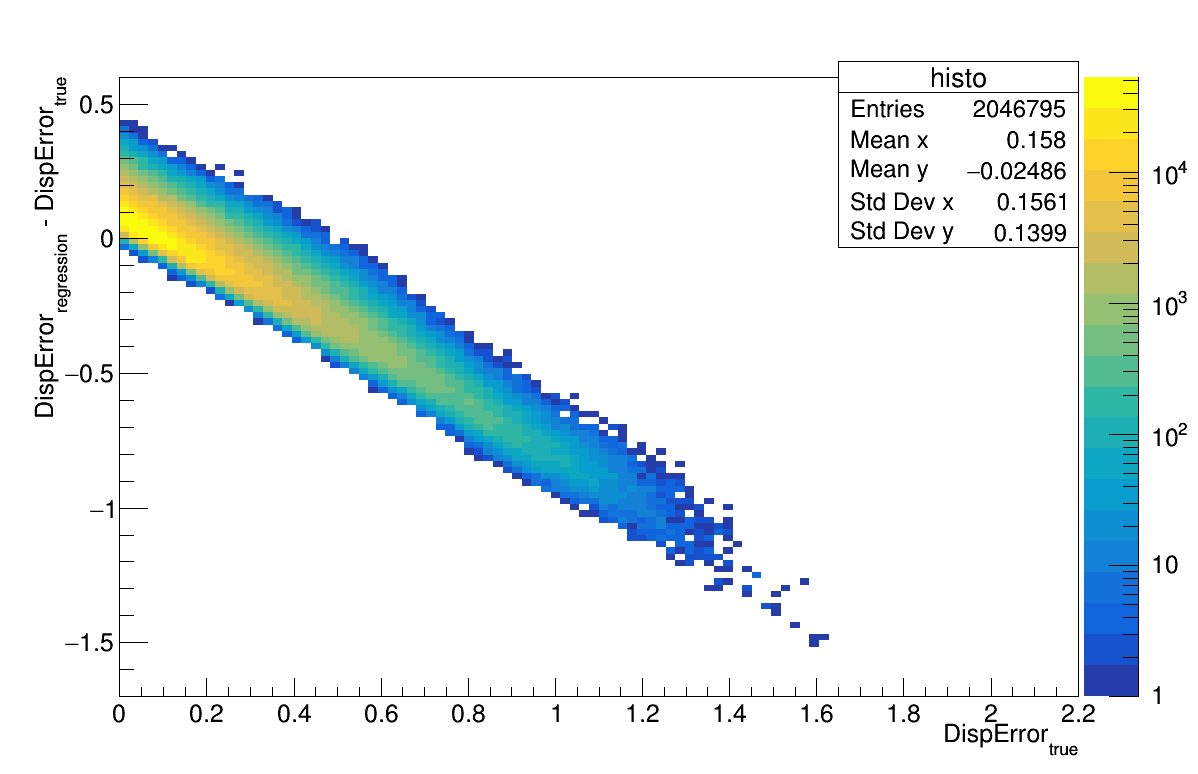
\includegraphics[width=.47\linewidth]{DispError_Train}
    \label{fig:dispErr_train_overtraining}
  }
  \subfigure[Deviation of reconstructed \disp Error parameter from Monte-Carlo \disp Error parameter in testing sample.]{
    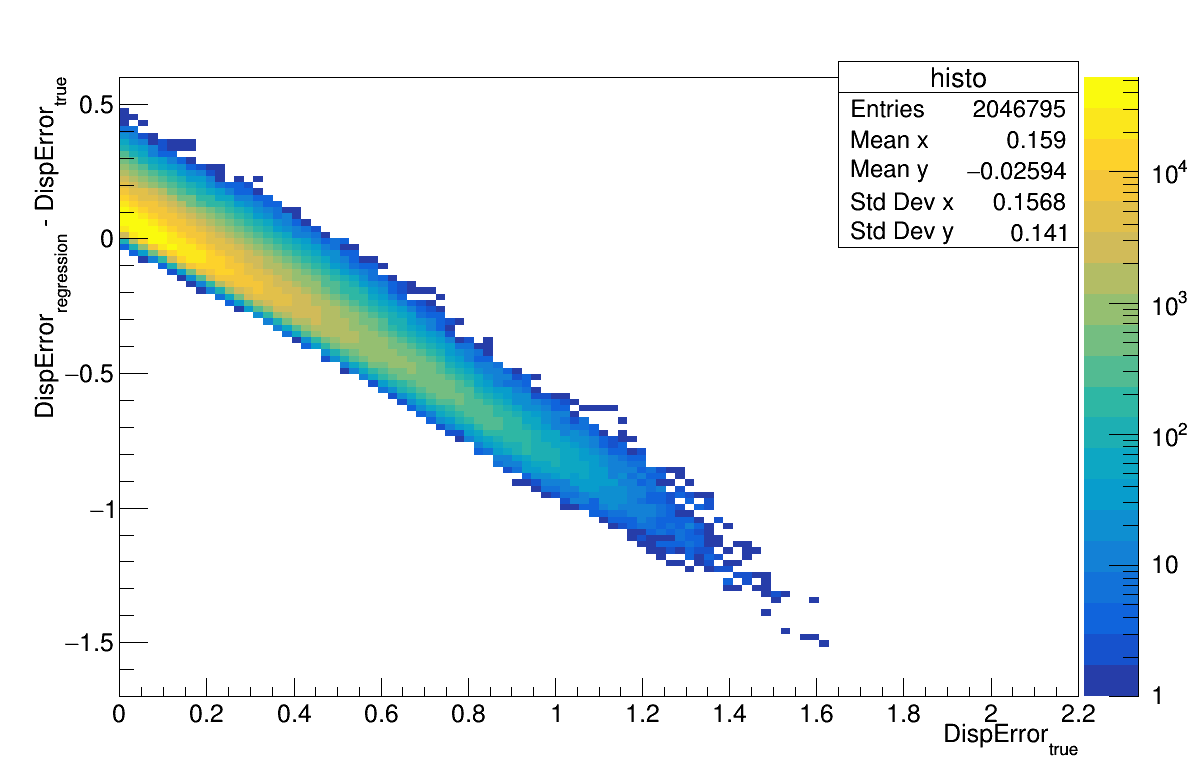
\includegraphics[width=.47\linewidth]{DispError_Test}
    \label{fig:dispErr_test_overtraining}
  }
  \subfigure[Deviation of reconstructed MAError parameter from Monte-Carlo MAError parameter in training sample.]{
    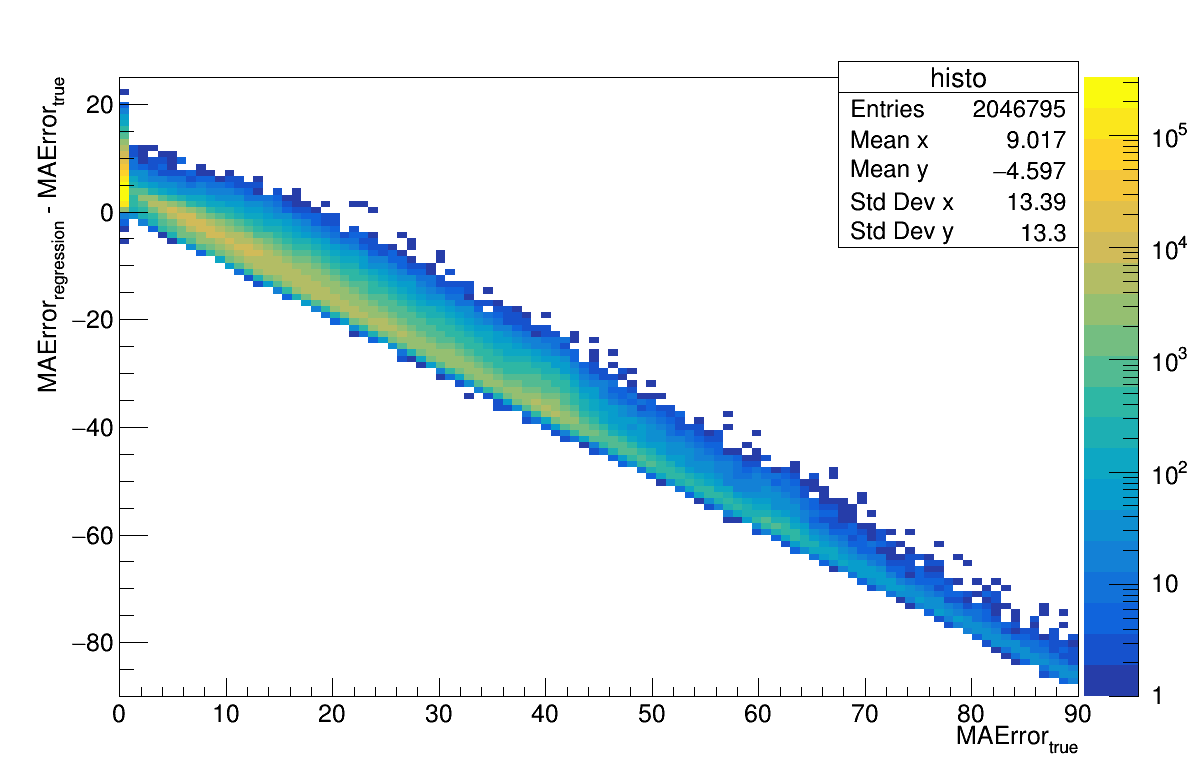
\includegraphics[width=.47\linewidth]{MAError_Train}
    \label{fig:MAErr_train_overtraining}
  }
  \subfigure[Deviation of reconstructed MAError parameter from Monte-Carlo MAError parameter in testing sample.]{
    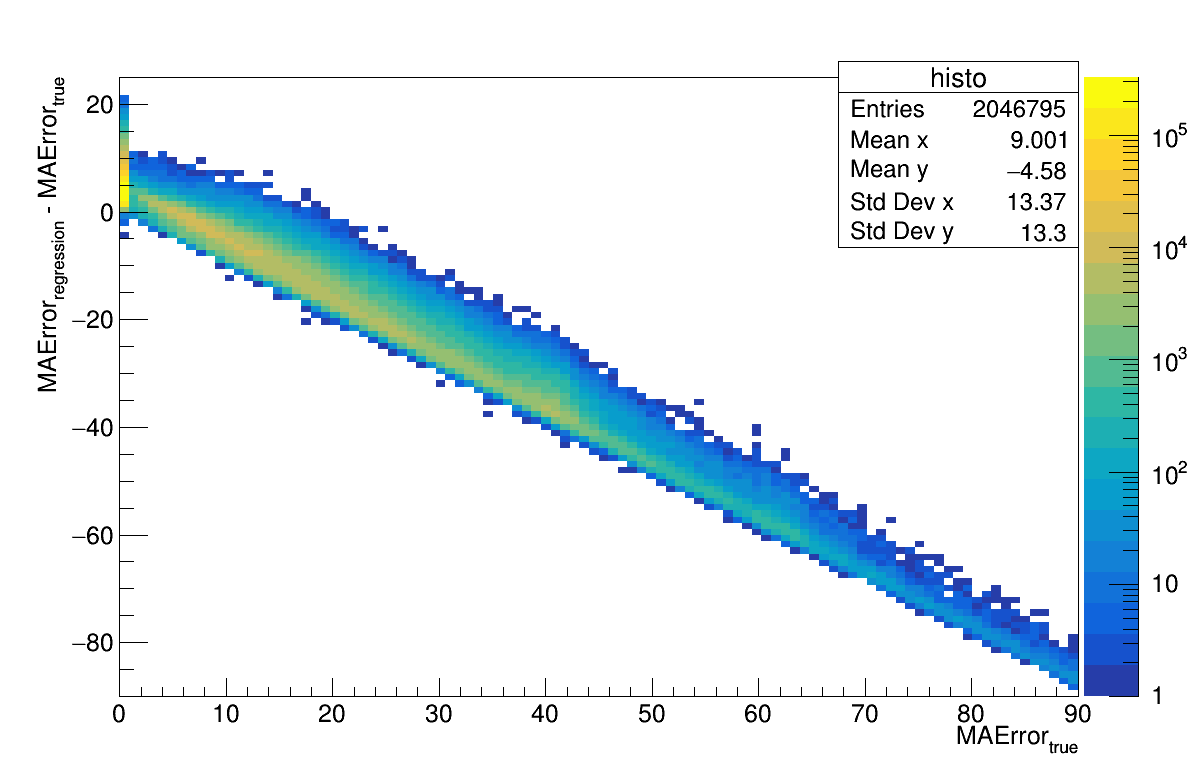
\includegraphics[width=.47\linewidth]{MAError_Test}
    \label{fig:MAErr_test_overtraining}
  }
  \caption[Over-training test.]{Over-training check on reconstruction using a \disp table generated at a single noise level. The left column shows the deviation of the reconstructed parameter from the true value in the training sample and the column on the right shows the same in the testing sample. The difference between the two columns is small which suggests there is little or no overtraining.}
  \label{fig:overtraining}
\end{figure}

\subsection{Noise Related Effects}
The first set of \disp tables was also generated at a single noise level ($250$ MHz), allowing us to test the dependence of the resolution of this method (as measured by R$_{68}$) on noise level in the testing sample -- some kind of noise-dependent effect would suggest over-training that would not be evident from the testing sample in the ROOT TMVA method since all the data provided to the package would have been at the same noise level. A comparison of angular resolution across noise levels revealed no significant dependence of the \rse on noise (see Fig. \ref{fig:olddisp_ratio}, \ref{fig:disp_ratio_250} and \ref{fig:disp_ratio_450}).

\begin{figure}[htbp]
  \centering
  \subfigure[Numerically determined R$_{68}$.]{
    \includegraphics[width=.8\linewidth]{num/disp_450_ratio_xzen}
    \label{fig:disp_ratio_450_num}
  }
  \subfigure[R$_{68}$ as determined from a fit.]{
    \includegraphics[width=0.8\linewidth]{fit/disp_450_ratio_xzen}
    \label{fig:disp_ratio_450_fit}
  }

  \caption[\disp table reconstruction vs noise.]{Ratio of \rse of the noise=450MHz \disp table ($\sim 2.1\e6$ events) to that from Method0 with the numerically determined \rse (left) and that found from the fit to two Gaussians (right). Note that the result is largely independent of the noise level in the simulation sample being reconstructed.}
  \label{fig:disp_ratio_450}
\end{figure}

A second set of test \disp tables was generated using a single noise level (noise $= 450$ MHz) to test for over-training related to noise in the training sample (see Fig. \ref{fig:disp_ratio_450}). These tables performed slightly better than the first test tables and comparably to the standard \disp tables, but not significantly so. Since the noise-related effects did not seem to play a significant role in reconstruction, noise was dropped as a discriminating parameter for further analysis. Together, these two tests confirm that we do not expect the \disp method reconstruction to be dependent on the noise levels in either the training sample or the data being reconstructed and therefore this reconstruction should not be sensitive to different NSB models.

To generate a set of \disp tables with better angular resolution (as measured by \rse\hspace{-4pt}), another set of \disp tables was trained on a larger number of simulations across zenith angles (as before) as well as across the noise spectrum. Since noise was determined not to impact the reconstruction, the events at different noise levels were used only to create samples with greater statistics.

\subsection{Higher Statistics Tables}
Once it was determined that there was no significant over-training in the small sample \disp tables, and the noise level had little bearing on the \rse measure of the reconstruction, it was determined that different noise level simulation events could be used as independent training events to have a higher statistics \disp table, and make small improvements on the statistical uncertainty on the reconstruction. The simulation data from across the noise spectrum and zenith range was used to generate a \disp table that sampled the entire parameter space more exhaustively.

A new set of \disp tables was generated (Fig. \ref{fig:disp_ratio_450x4}) with a training sample four times that of the initial test tables. The improvements in resolution due to change in sample size were modest, and confined to the range of zenith angles (zenith $>45^\circ$) where the standard method outperforms the \disp method quite considerably.

\begin{figure}[htbp]
  \centering
  \subfigure[Numerically determined R$_{68}$.]{
    \includegraphics[width=0.8\linewidth]{num/disp_450x4size_ratio_xzen}
    \label{fig:disp_ratio_450x4_num}
  }
  \subfigure[R$_{68}$ as determined from a fit.]{
    \includegraphics[width=0.8\linewidth]{fit/disp_450x4size_ratio_xzen}
    \label{fig:disp_ratio_450x4_fit}
  }
  \caption[Higher statistics \disp table reconstruction vs noise.]{Ratio of \rse of the noise=450MHz \disp table ($\sim 8.4\e6$ events) to that from Method0 for a higher statistics \disp table with the numerically determined \rse (left) and that found from the fit to two Gaussians (right).}
  \label{fig:disp_ratio_450x4}
\end{figure}

As expected from the small statistical uncertainty on the \rse values, this increase in sample size did not lead to any meaningful improvements and a training sample of $\sim 2\e6$ was determined to be sufficient to achieve the desired resolution with small uncertainties.

\subsection{Acceptance Correction for Offset from Camera Center}
Showers arriving further from the camera center have a larger fraction of the shower arriving outside of the camera and therefore being lost. These showers are therefore reconstructed with a lower efficiency and resolution than showers arriving closer to the camera center. To compensate for this in the BDT training, so that the training sample does not mis-characterize the overabundance of events closer to the camera center as an anisotropy in incoming gamma rays, we fold in an acceptance correction by assigning a larger weight to events that are further away from the camera center.

The acceptance correction used here affects the training sample and therefore might be assumed to affect the resolution in a zenith dependent way, perhaps explaining the difference in performance between the new \disp tables and the old ones. This was tested by using a number of different correction functions in the training sample, as shown in Fig. \ref{fig:weights}

\begin{figure}[htbp]
  \centering
  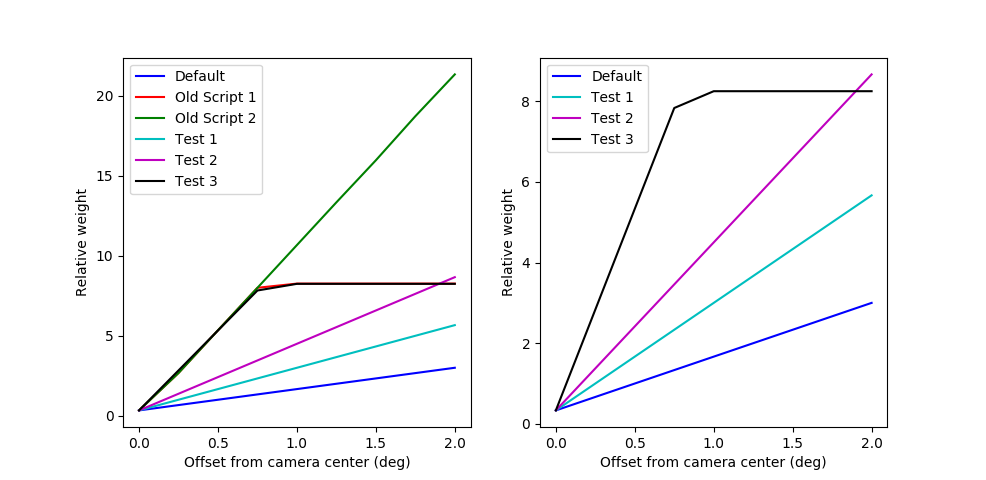
\includegraphics[width=.78\linewidth]{weights}
  \caption[Weight functions for offset from camera center.]{The weight functions used in the training samples in the new tables (Default, Test 1, Test 2 and Test 3) and those found in the scripts used to generate the older tables (Old Script 1, Old Script 2).}
  \label{fig:weights}
\end{figure}

These tests reveal small changes in the \rse value despite large changes in the correction function (Fig. \ref{fig:weight_tests}). This suggests that the \disp tables are not sensitive to changes in acceptance and therefore the different acceptance functions are unlikely to be the reason why the new \disp tables perform worse at smaller zenith angles.

\begin{figure}[H]
  \centering
  \subfigure[Numerically determined R$_{68}$.]{
    \includegraphics[width=.75\linewidth]{num/disp_wts}
    \label{fig:weight_tests_num}
  }
  \subfigure[R$_{68}$ as determined from a fit.]{
    \includegraphics[width=.75\linewidth]{fit/disp_wts}
    \label{fig:weight_tests_num}
  }
  \caption[\rse for the acceptance correction functions.]{\rse for each acceptance correction function shown in Fig. \ref{fig:weights} with the numerically determined \rse (left) and that found from the fit to two Gaussians (right). The changes in acceptance correction do not meaningfully change the \rse for the reconstruction.}
  \label{fig:weight_tests}
\end{figure}

\subsection{Energy Dependence}
Another important dependence of the reconstruction resolution (and therefore the R$_{68}$) is that on energy. Higher energy photons are expected to comprise a larger fraction of LZA photons because lower energy showers suffer more absorption in the atmosphere. Conversely, high energy photons make up a small fraction of SZA photons (and more generally, all cosmic photons) due to the $\sim E^{-2}$ shape of the spectrum. A better resolution at higher energy would also be expected to contribute to the improved resolution at LZA.

Due to the slicing in energy in addition to zenith and therefore smaller number statistics, this is expected to lead to relatively sparse data in each bin. For this reason, in this section we address only the \rse determined from the numerical integral, and not that from the fit.

\begin{figure}[htbp]
  \centering
  \subfigure[Energy Dependence of Method0 at small and medium zenith angles.]{
    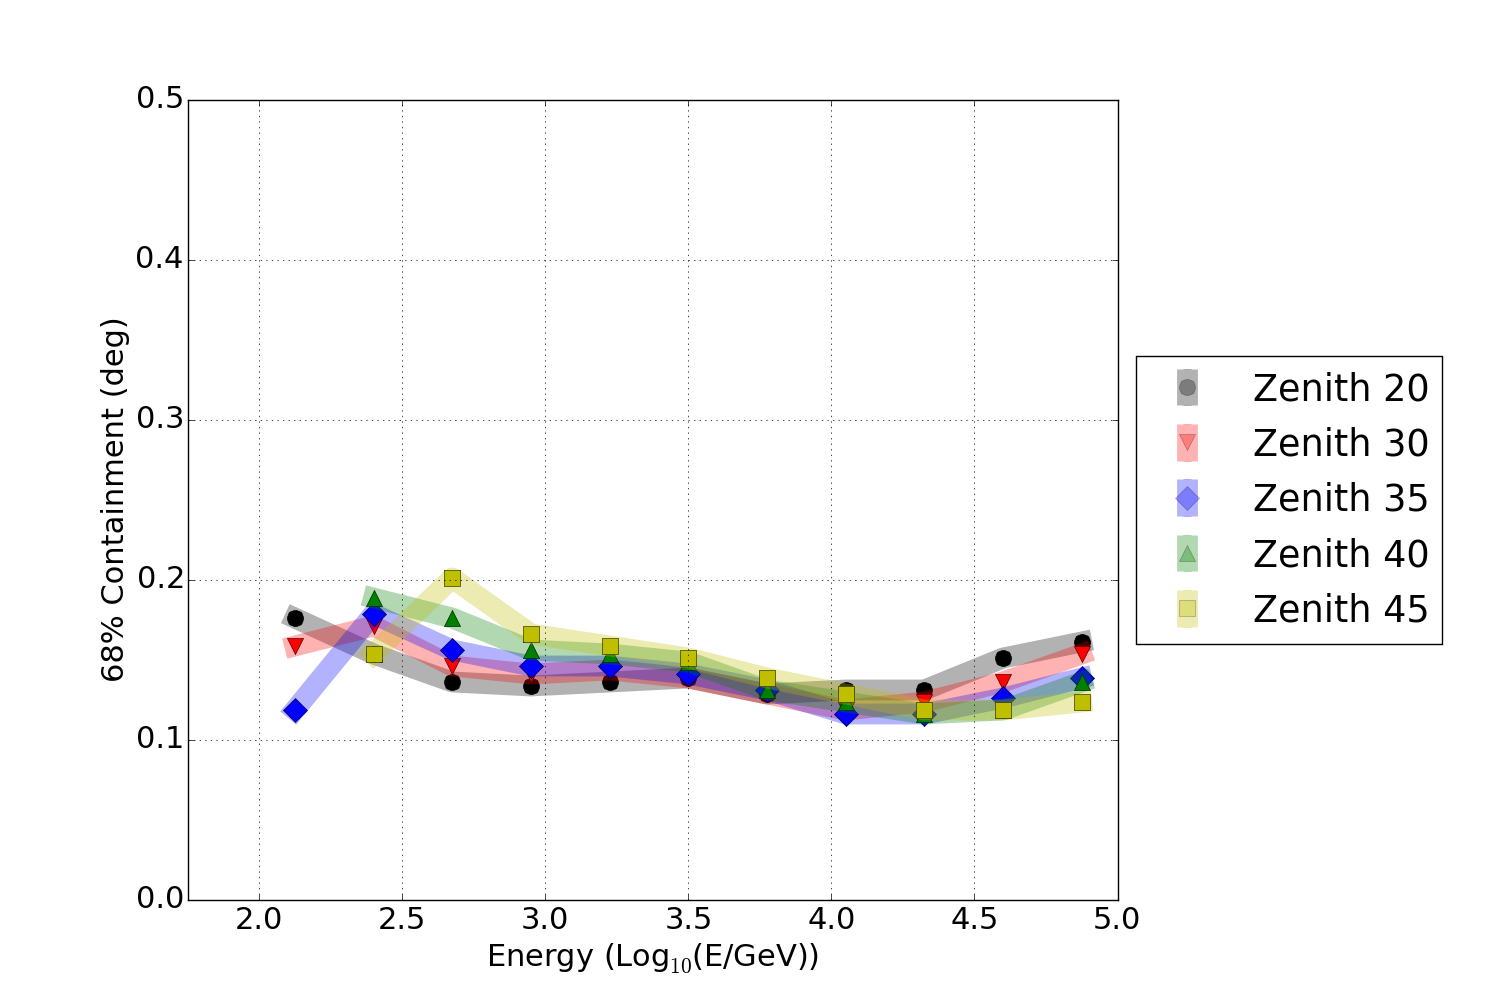
\includegraphics[width=.44\linewidth]{num/reg_SZA_energy}
    \label{fig:energy_reg_SZA}
  }
  \subfigure[Energy Dependence of Method0 at large zenith angles.]{
    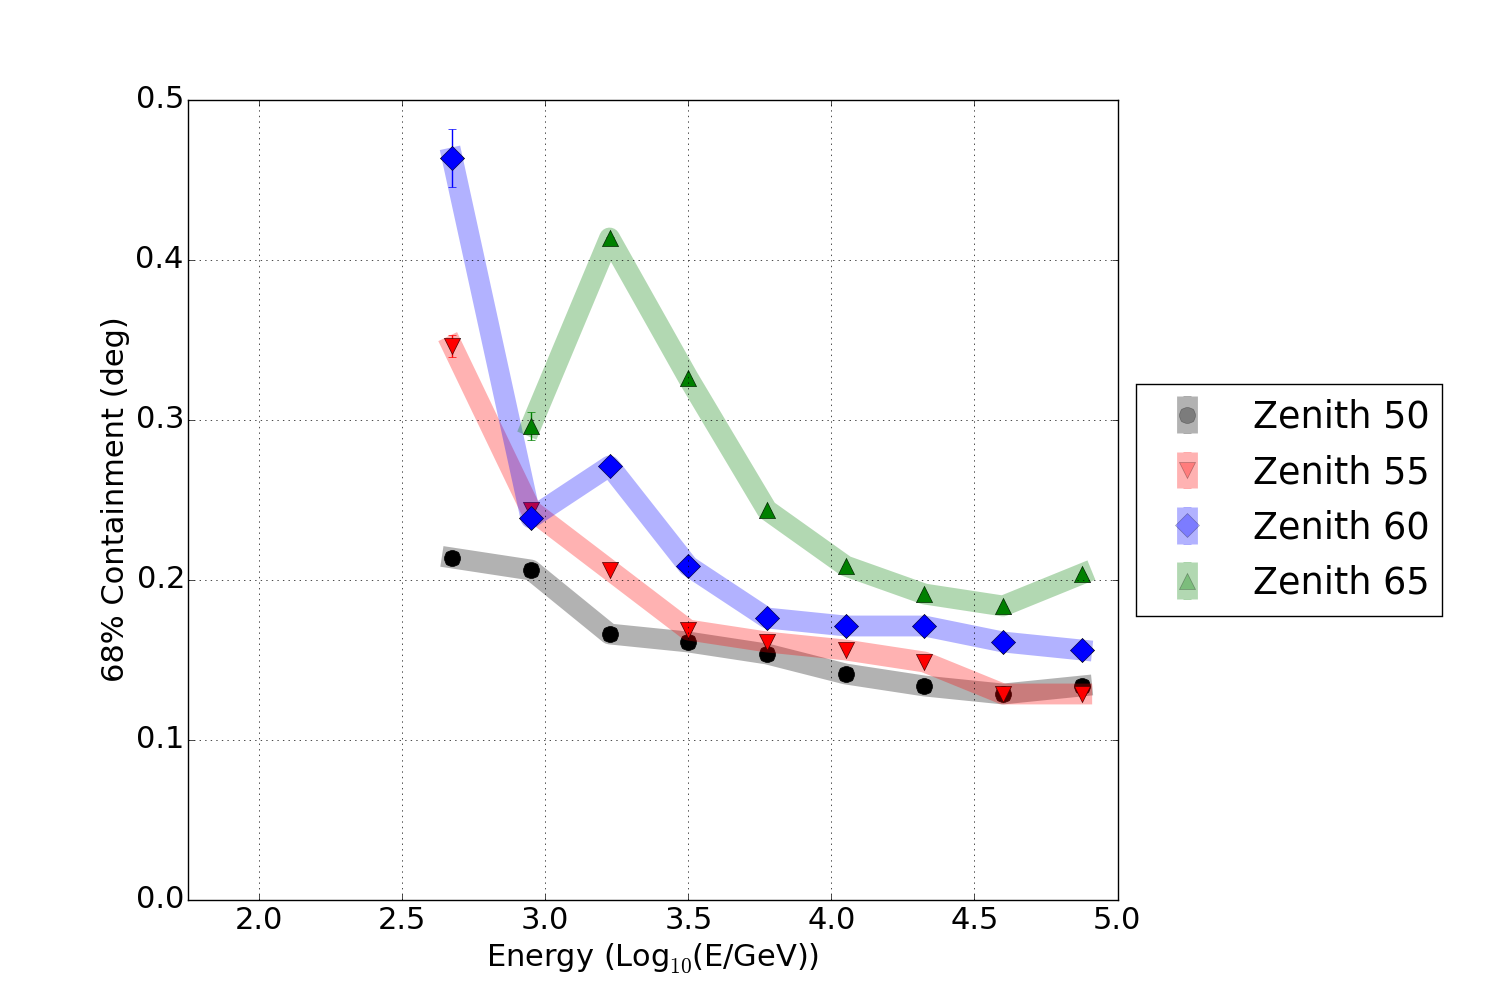
\includegraphics[width=.44\linewidth]{num/reg_LZA_energy}
    \label{fig:energy_reg_LZA}
  }
  \caption[Energy Dependence of Method0.]{Energy Dependence of Method0 with \rse for small zenith angles (left) and that for large zenith angles (right). Colored bands are intended to guide the eye and do not represent data points.}
  \label{fig:energy_reg}
\end{figure}

\begin{figure}[htbp]
  \centering
  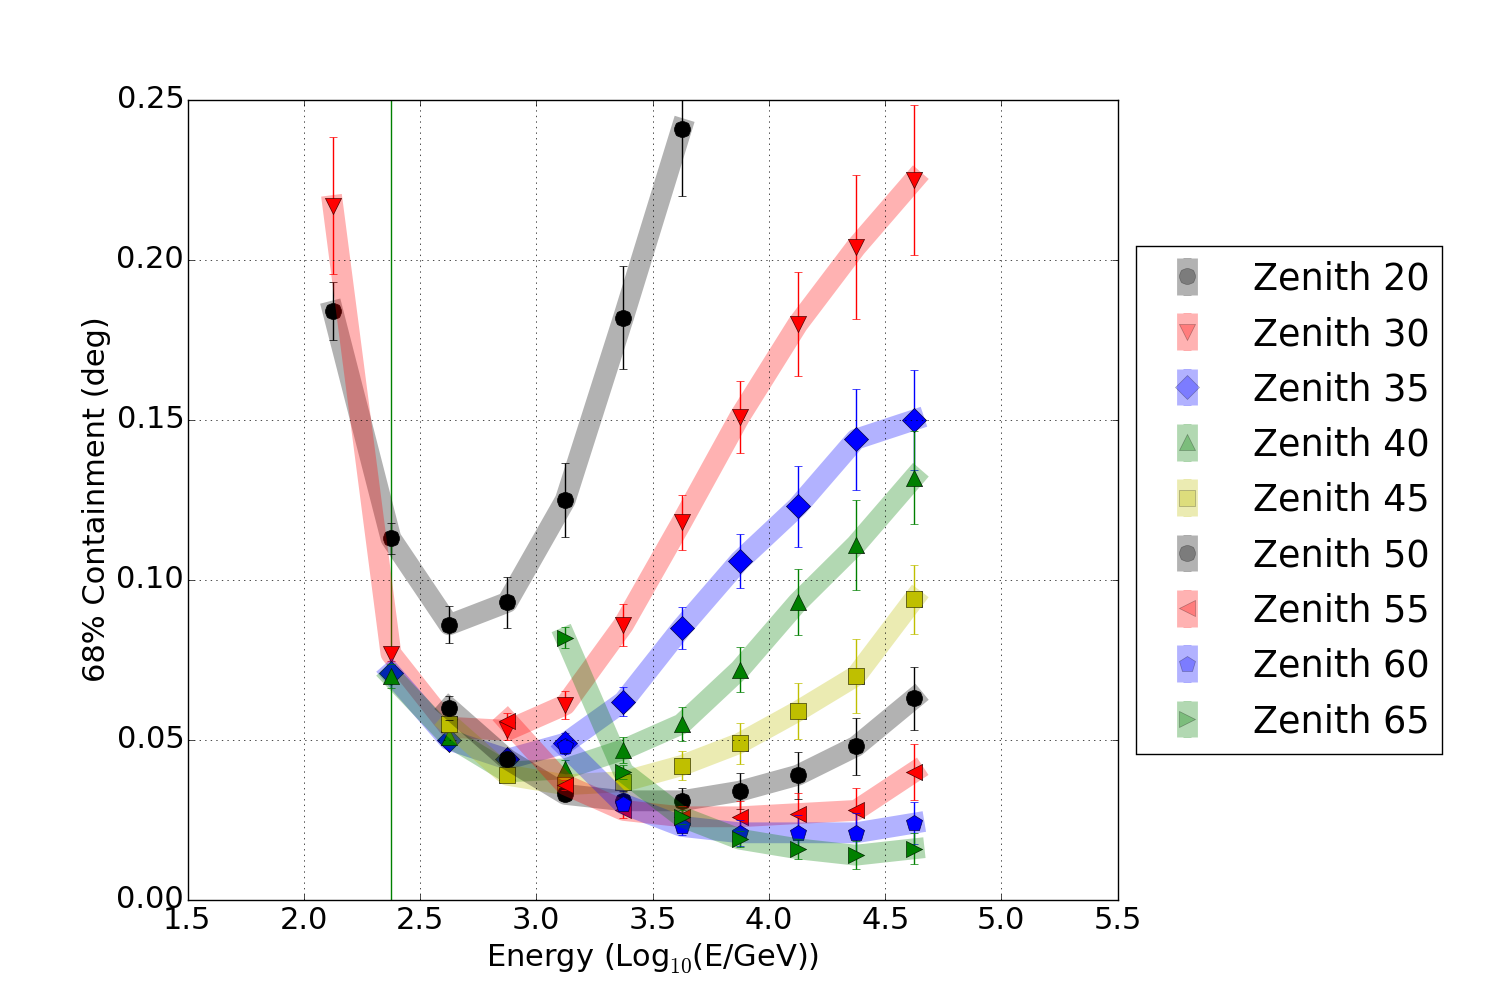
\includegraphics[width=.75\linewidth]{num/disp_standard_energy}
  \caption[Energy Dependence of the old Method5t.]{Energy Dependence of the old Method5t with the numerically determined \rse (left) and that found from the fit to two Gaussians (right). Colored bands are intended to guide the eye and do not represent data points.}
  \label{fig:energy_disp_standard}    
\end{figure}

\begin{figure}[htbp]
  \centering
  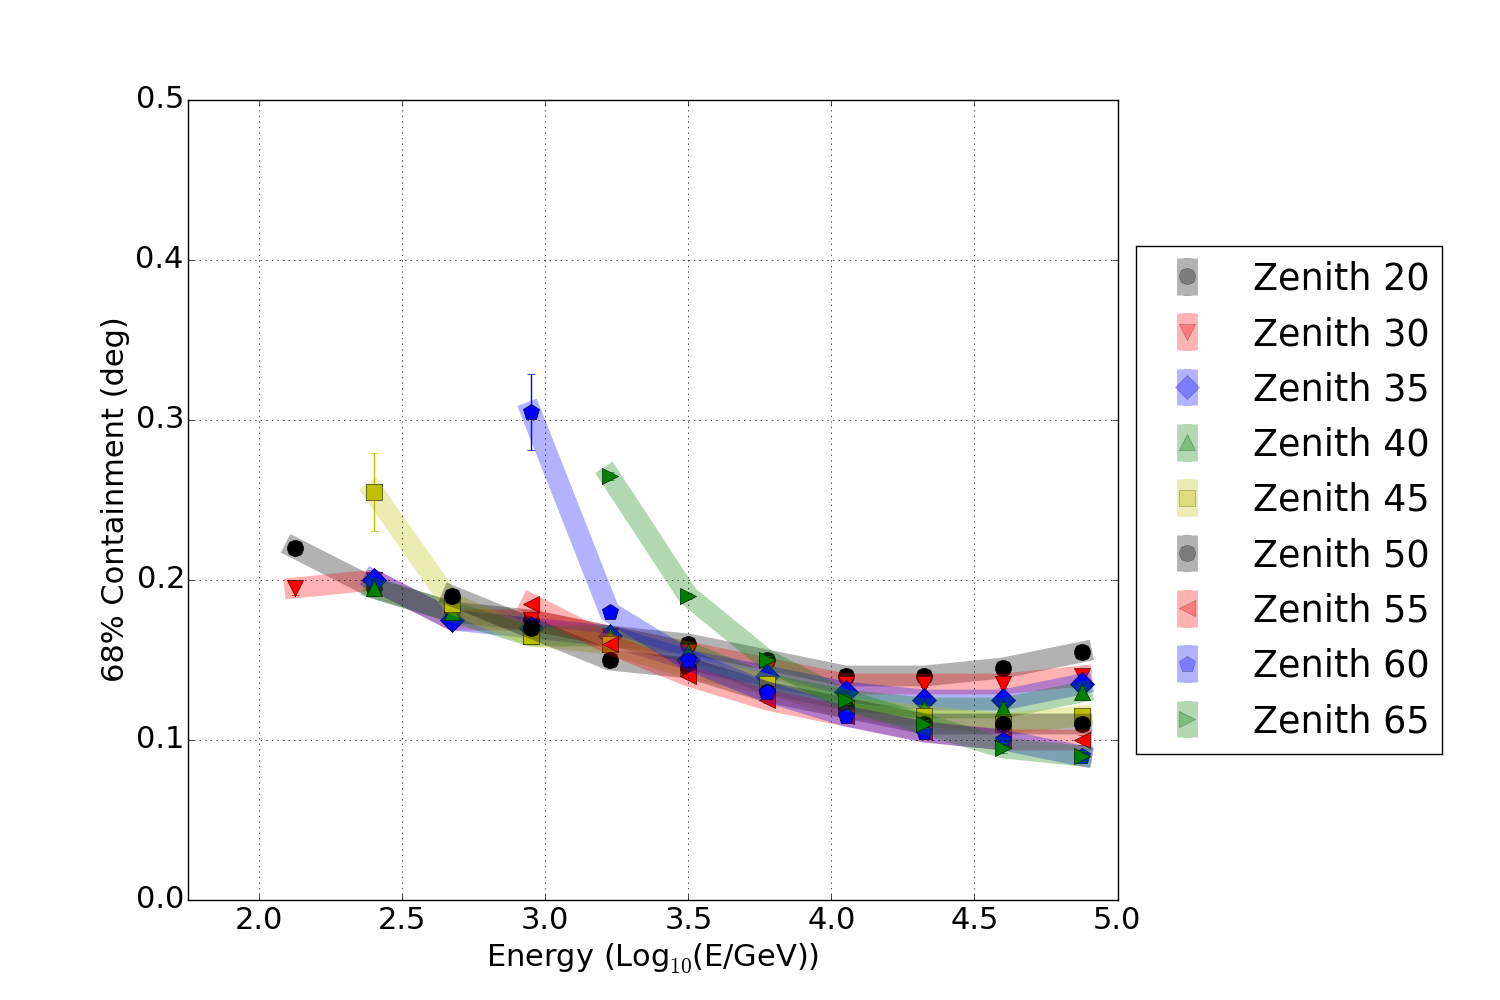
\includegraphics[width=.75\linewidth]{num/disp_450x4size_energy}
  \caption[Energy Dependence of the new Method5t.]{Energy Dependence of the new Method5t with the numerically determined \rse (left) and that found from the fit to two Gaussians (right). Colored bands intended to guide the eye and do not represent data points.}
  \label{fig:energy_disp_450}    
\end{figure}

The Method0 energy dependence (Fig. \ref{fig:energy_reg}) follows the same trend as in Fig. \ref{fig:disp_res} -- seeing the best resolution for all zenith angles in the 3-30TeV range as well as a low energy improvement likely driven by higher statistics. The energy dependence for the older \disp tables (Fig. \ref{fig:energy_disp_standard}) appears to have a minimum in \rse close to 1 TeV. These old \disp tables also see a degradation in resolution at the highest energies. The newer \disp tables (Fig. \ref{fig:energy_disp_450}) on the other hand appear to do {\bf better at higher energies for all zenith angles}. At energies above $\sim 1$ TeV and zenith angle greater than $30^\circ$, the \rse is at or better than $0.3^\circ$ (see Fig. \ref{fig:energy_new_contour}). Compared to the geometric method this provides major improvements in the LZA region (top rows of Fig. \ref{fig:reg_rse} and \ref{fig:reg_sim}) and compared to the older \disp tables, we see major improvements in the high energy-medium zenith regime (lower right corner of Fig. \ref{fig:disp_standard_rse} and \ref{fig:disp_standard_sim})

\begin{figure}[htbp]
  \centering
  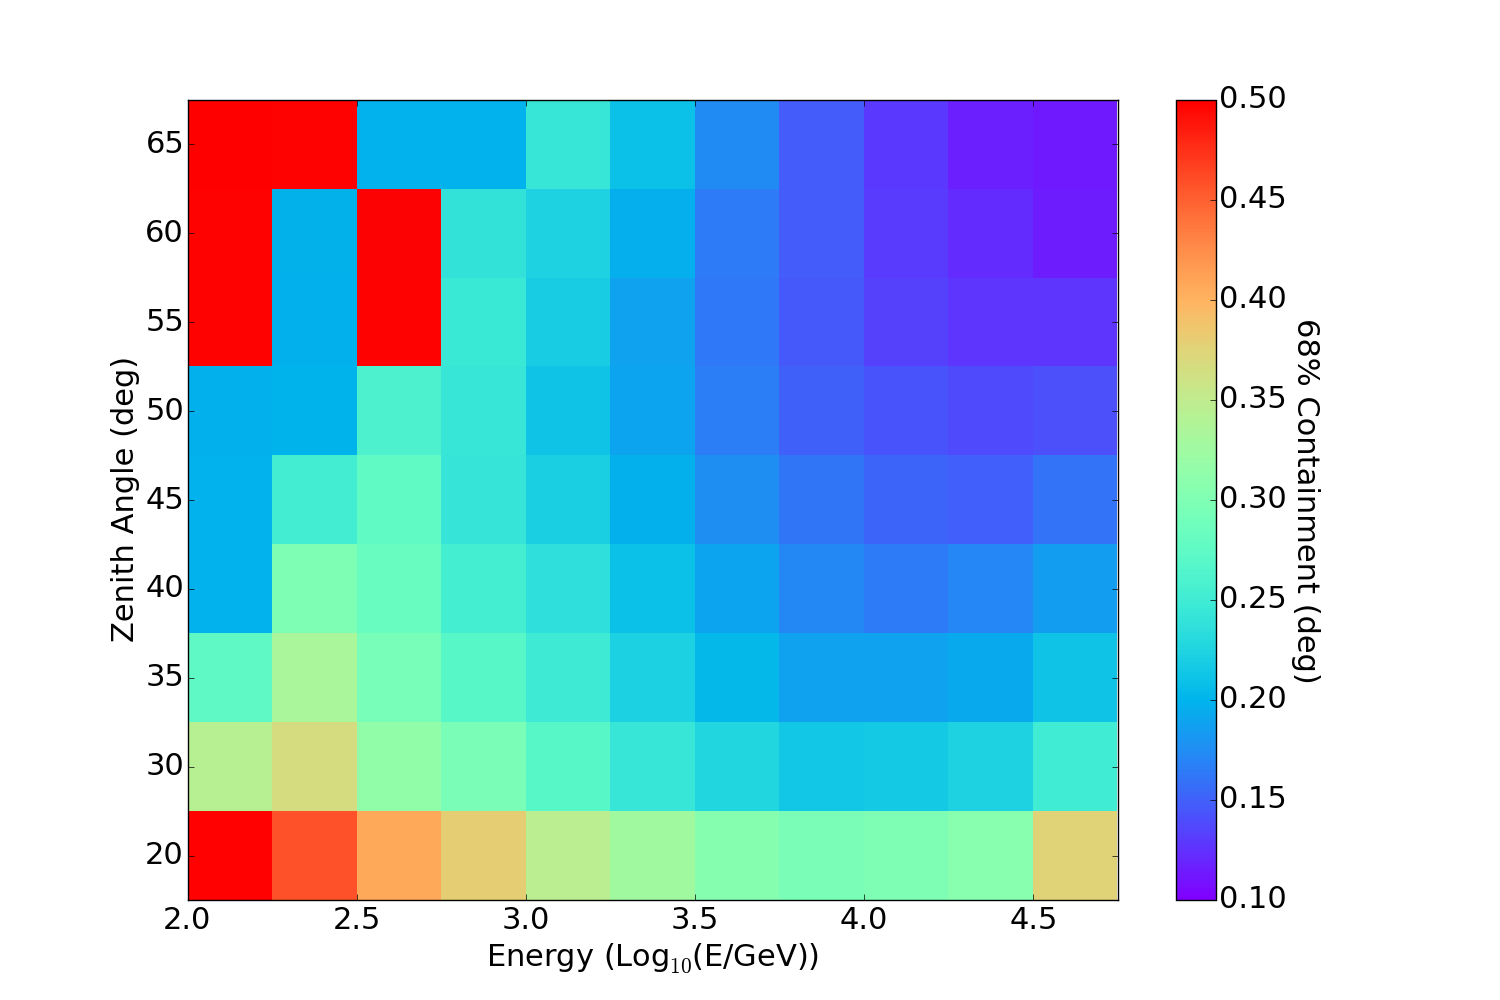
\includegraphics[width=.9\linewidth]{num/disp_450x4size_rse}
  \caption[Energy and zenith dependence of the new Method5t.]{Energy and zenith dependence of the new Method5t, with colors denoting the \rse and red denoting \rse$\geq0.50^\circ$. The upper-left corner shows regions of loss in resolution in the large-zenith low-energy region due to low statistics.}
  \label{fig:energy_new_contour}
\end{figure}

\begin{figure}[htbp]
  \centering
  \subfigure{
    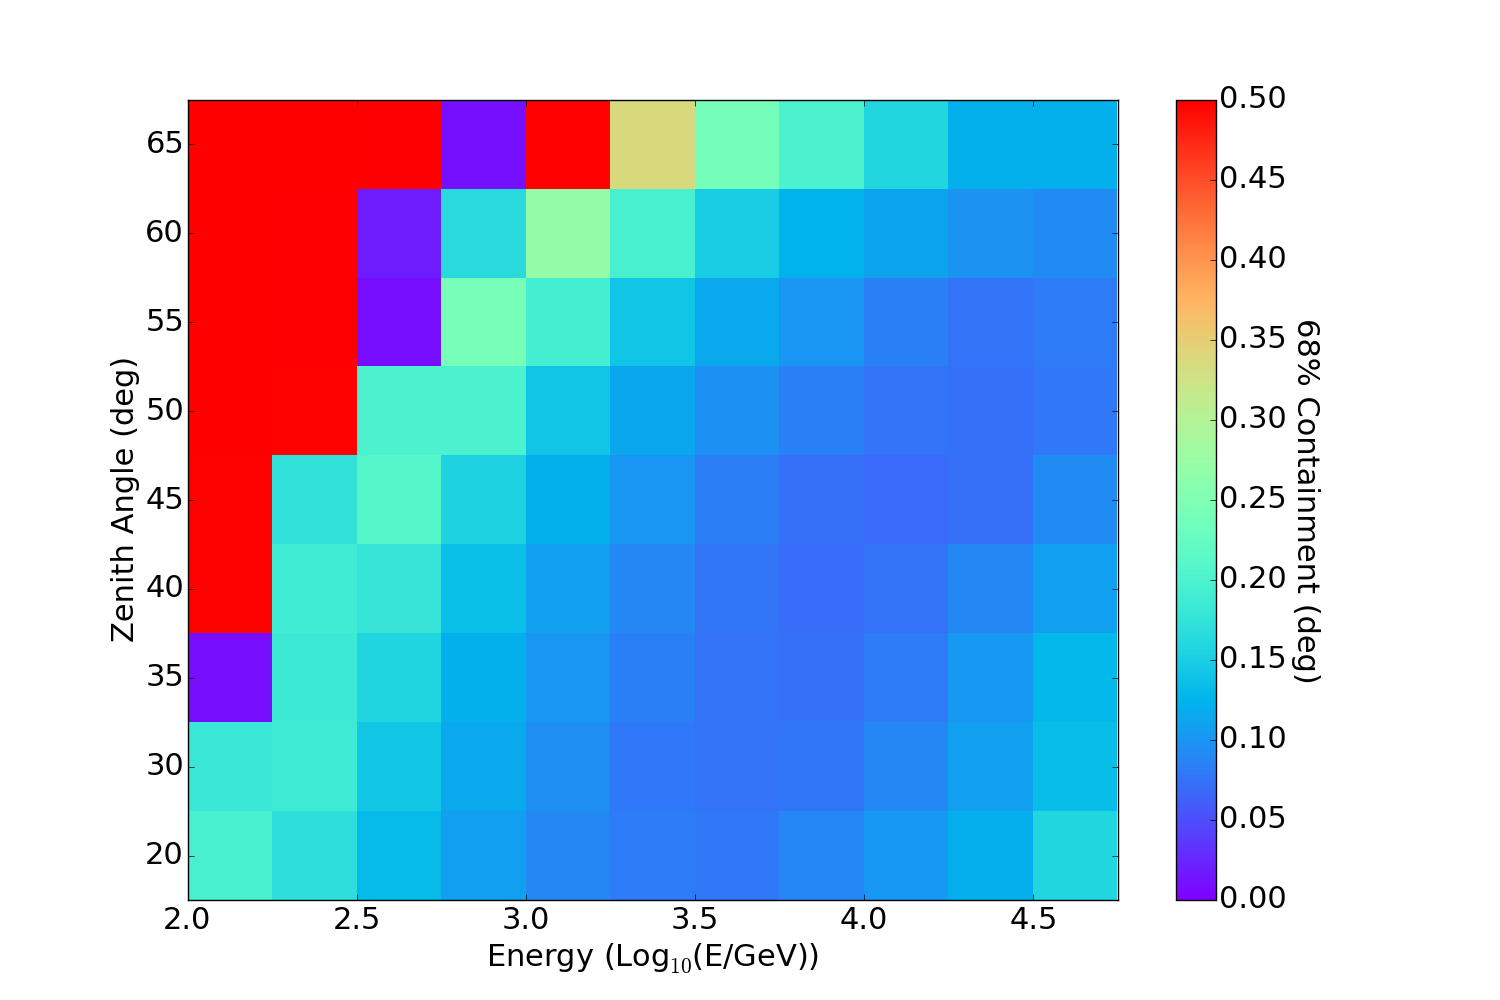
\includegraphics[width=0.47\linewidth]{num/reg_rse}
    \label{fig:reg_rse}
  }
  \subfigure{
    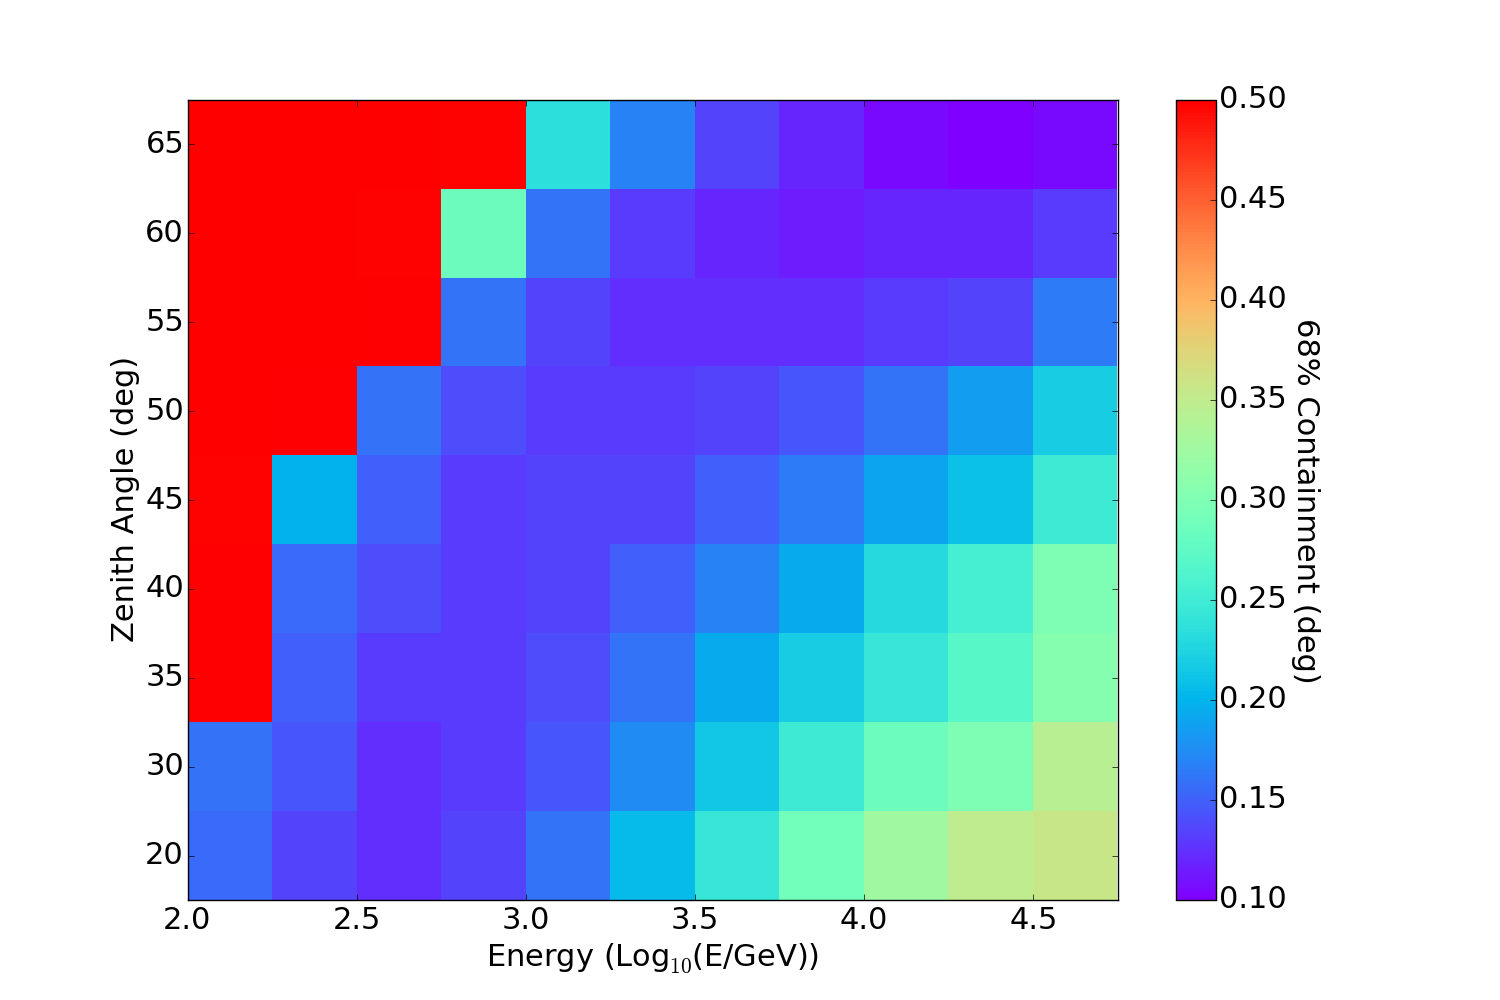
\includegraphics[width=0.47\linewidth]{num/disp_standard_rse}
    \label{fig:disp_standard_rse}
  }
  \caption[Energy and zenith dependence of Method0 and the old Method5t]{Energy and zenith dependence of the geometric reconstruction (left) and the old Method5t (right), with colors denoting the \rse and red denoting \rse$\geq0.50^\circ$.}
  \label{fig:energy_contour}
\end{figure}

\begin{figure}[htbp]
  \centering
  \subfigure{
    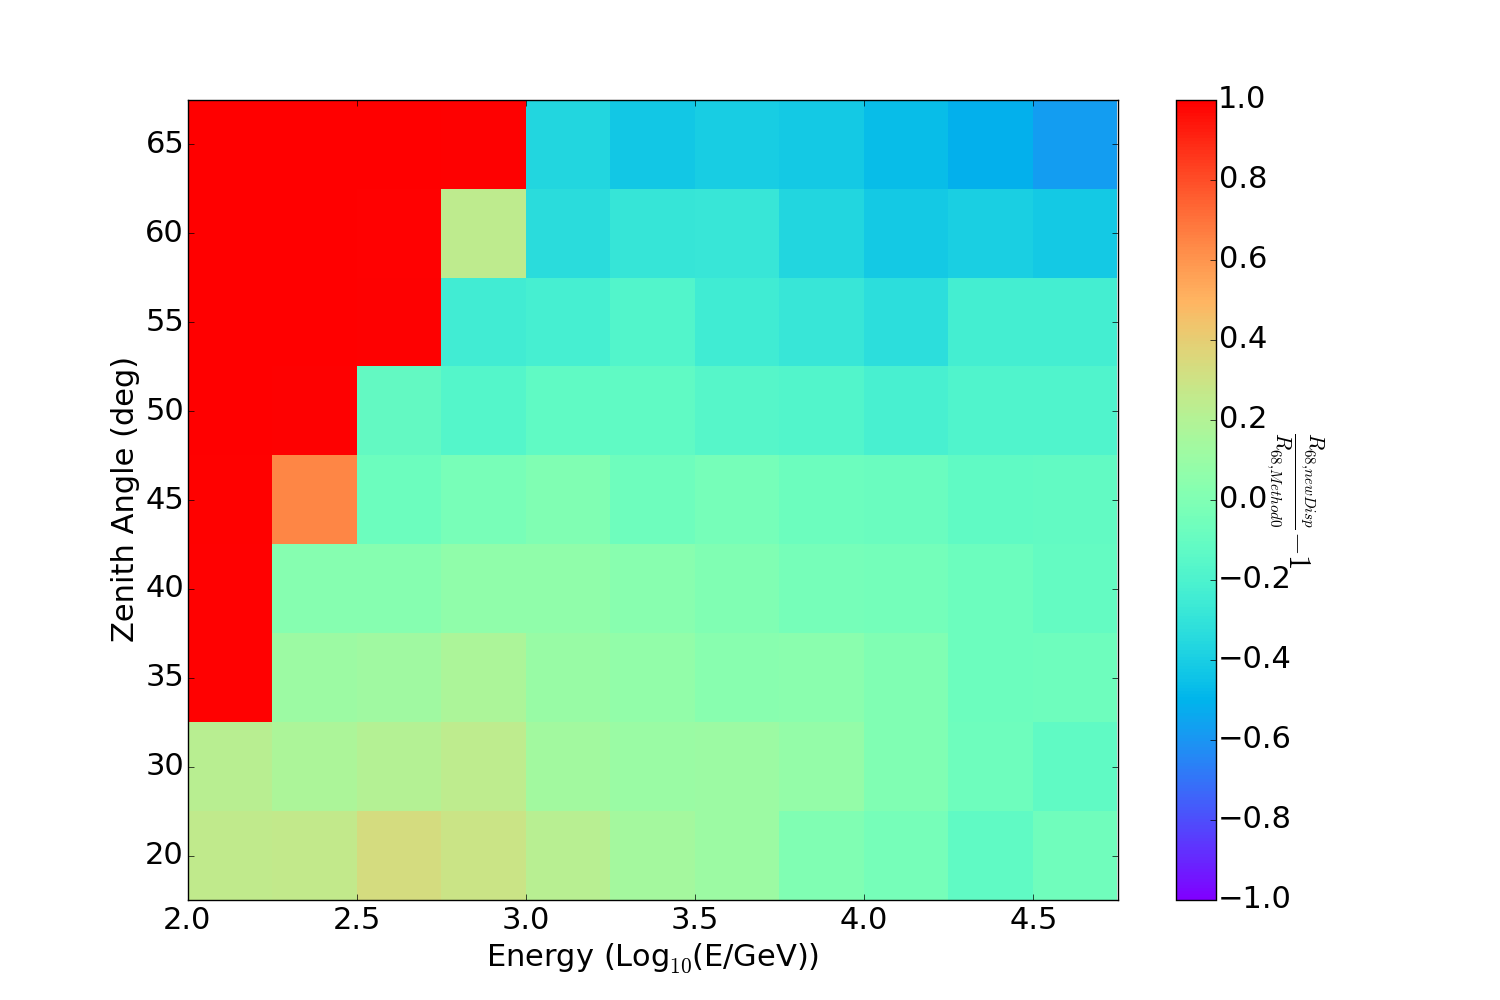
\includegraphics[width=0.47\linewidth]{num/rel_reg_sim}
    \label{fig:reg_sim}

  }
  \subfigure{
    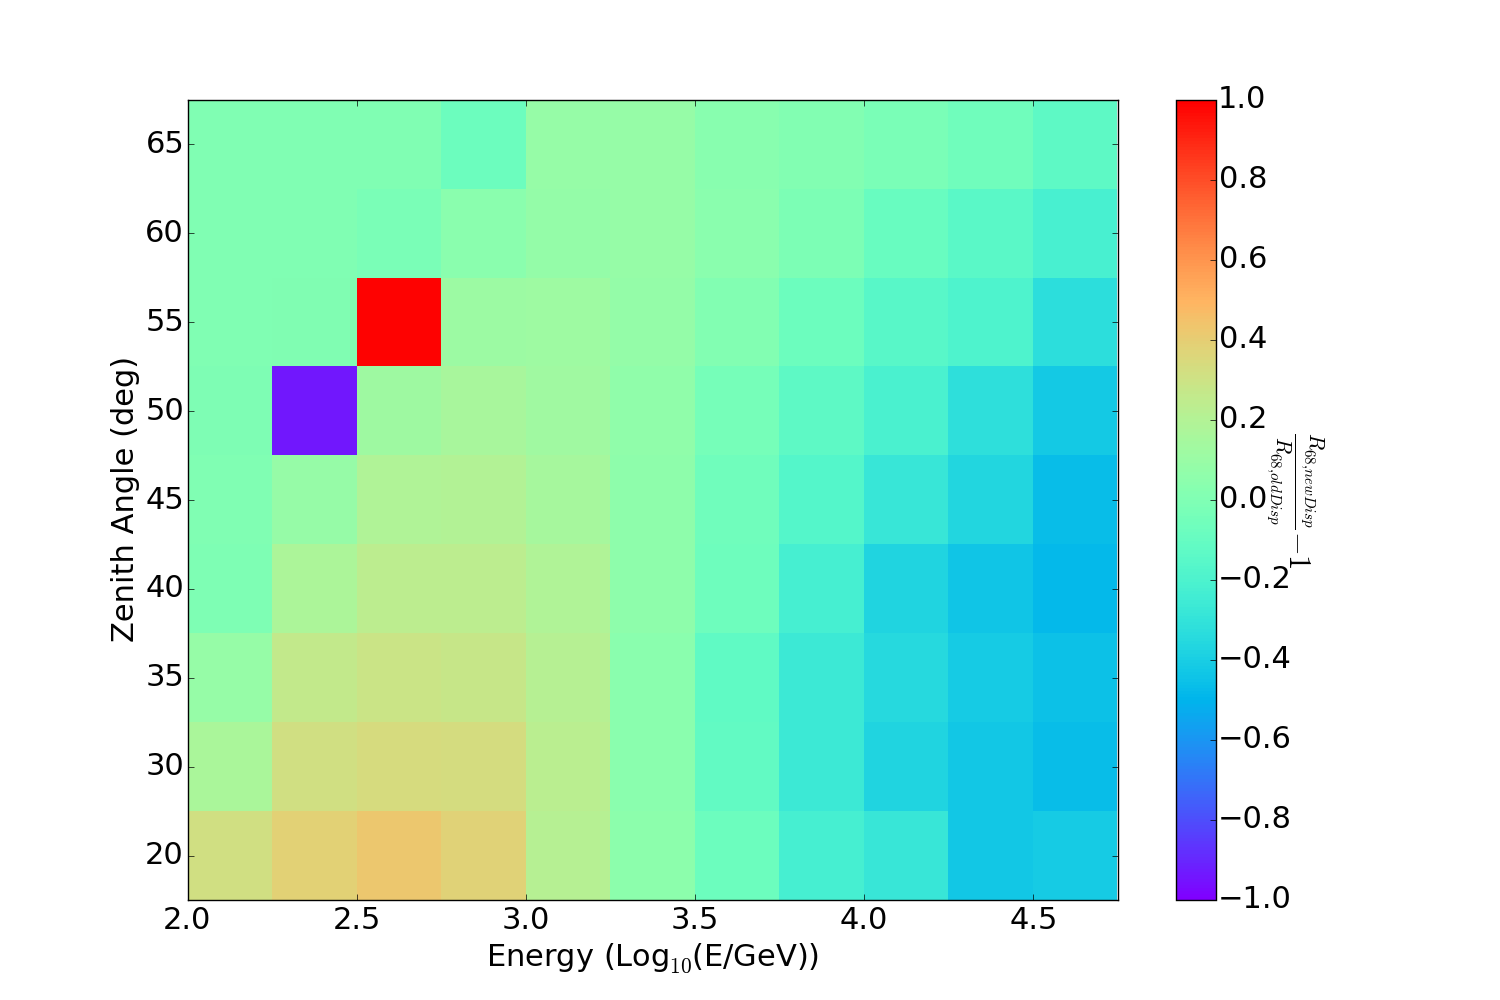
\includegraphics[width=0.47\linewidth]{num/rel_standard_sim}
    \label{fig:disp_standard_sim}
  }
  \caption[Performance of the new \disp method compared to Method0 and the old \disp method]{Performance of the new \disp method compared to Method0 (left) and the old \disp method (right), with purple at $-1.0$ denoting $100\%$ improvement over the older method and bright red (in the upper left corners) at $1.0$ denoting $100\%$ worse performance in that bin or regions of insufficient statistics. The range of usefulness for Method5t (relative to Method0) now extends to $E\geq1$TeV and $\phi\gtrsim55^\circ$ (upper left corner).}
  \label{fig:energy_rel}
\end{figure}

\section{\rse for Observational Data and Known Objects}
In order to test the validity of the results from the simulations, a known point-source with sufficient data collection at LZA and a hard spectrum (and therefore high statistics in the TeV range) was needed. Since our initial test was performed on the Crab Nebula and, in the VERITAS archival data it is the known object with the longest total exposure time at LZA, the Crab was used to generate some benchmarks. Additionally, Mrk421 was used as a known point source to test the power of discrimination between point and compact sources. Each of these objects and the corresponding analysis will be discussed in greater detail in the following sections.

\subsection{Data Constraints and Li \& Ma Significance}

For the data analysis, unlike with the simulations, a ``true'' direction was not knowable. Instead, the true direction must be assumed to be that of the known object, and we must restrict our analysis to those showers determined to be from the source object, and where the source object is in fact detected.

As a measure of detection, we use both the number of excess events -- defined as the number of events determined to be from the source over the number of events from the off-source regions scaled by the ratio of the exposures of the on and off-source regions. For a number of events from the source region is $N_{on}$, a number of events from the off-source region is $N_{off}$, and a ratio of exposure $\frac{A_{on}}{A_{off}}=\alpha$, the number of excess events is given by $N_{on}-\alpha N_{off}$. This corresponds to the number of events observed above the number expected given the background observation, and statements regarding the small- or large-number statistics refer to this number being small or large.

As a measure of the robustness of the \rse determined for the data, we also use the gamma-ray astronomy standard Li \& Ma\cite{LiMa} significance, with a threshold significance of $3\sigma$. A high significance measurement of the object in a given energy and zenith bin should provide a measure of \rse in that bin that is relatively stable against statistical fluctuations.

Lastly, as a measure of how the data analysis performs relative to expectations from the simulation analysis we also use a direct bin-wise comparison of the resulting numerical \rse defined as $\xi = \frac{R_{68, \text{data}}}{R_{68, \text{sim}}}-1$. This provides a numerical quantity that is expected to be zero and provides a simple percentage deviation from expectation. A $\xi$ of $0.3$ means the \rse from data in a given bin was 30\% larger than that from simulations, with positive values signifying ``under-performance'' and negative values signifying ``over-performance''.

\subsection{\rse for the Crab Nebula}

The Crab Nebula is measured to have a GeV-TeV extension of $\sim 0.03^\circ$ \cite{Fermi_LAT_Crab_extension}\cite{HESS_Crab_extension}. To observe this, a \rse of at least $0.03^\circ$ is required which, based on the simulations, we do not achieve (see Fig. \ref{fig:energy_disp_450}). This however provides another metric by which to quantify our resolution, as well as to measure possible future gains in resolution.

% Although this \rse is expected to be insufficient to \textit{measure} the GeV-TeV extension of the Crab due to low statistics, this can be used to demonstrate it \cite{Yeung:energy_extension}.

\begin{figure}[H]
  \begin{center}
    \subfigure[Angular resolution using Method5t.]{ 
      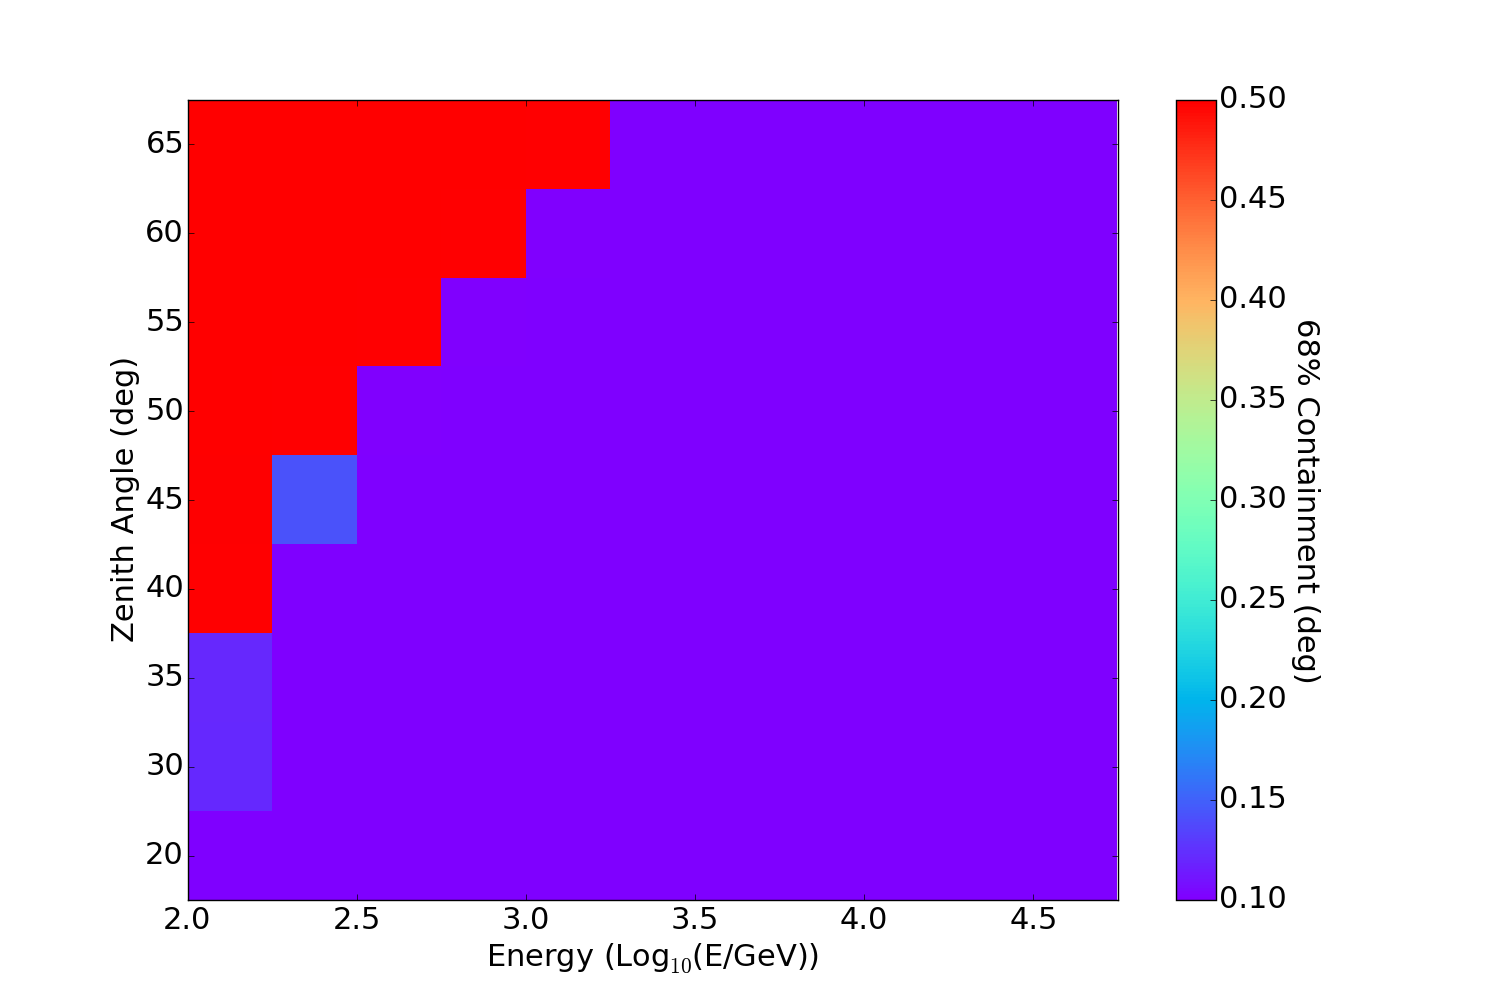
\includegraphics[width=0.47\linewidth]{num/LZA_data_25/crab_disp_rse.png}
      \label{fig:crab_disp_rse}
    }  
    \subfigure[Deviation from simulations ($\xi$).]{ 
      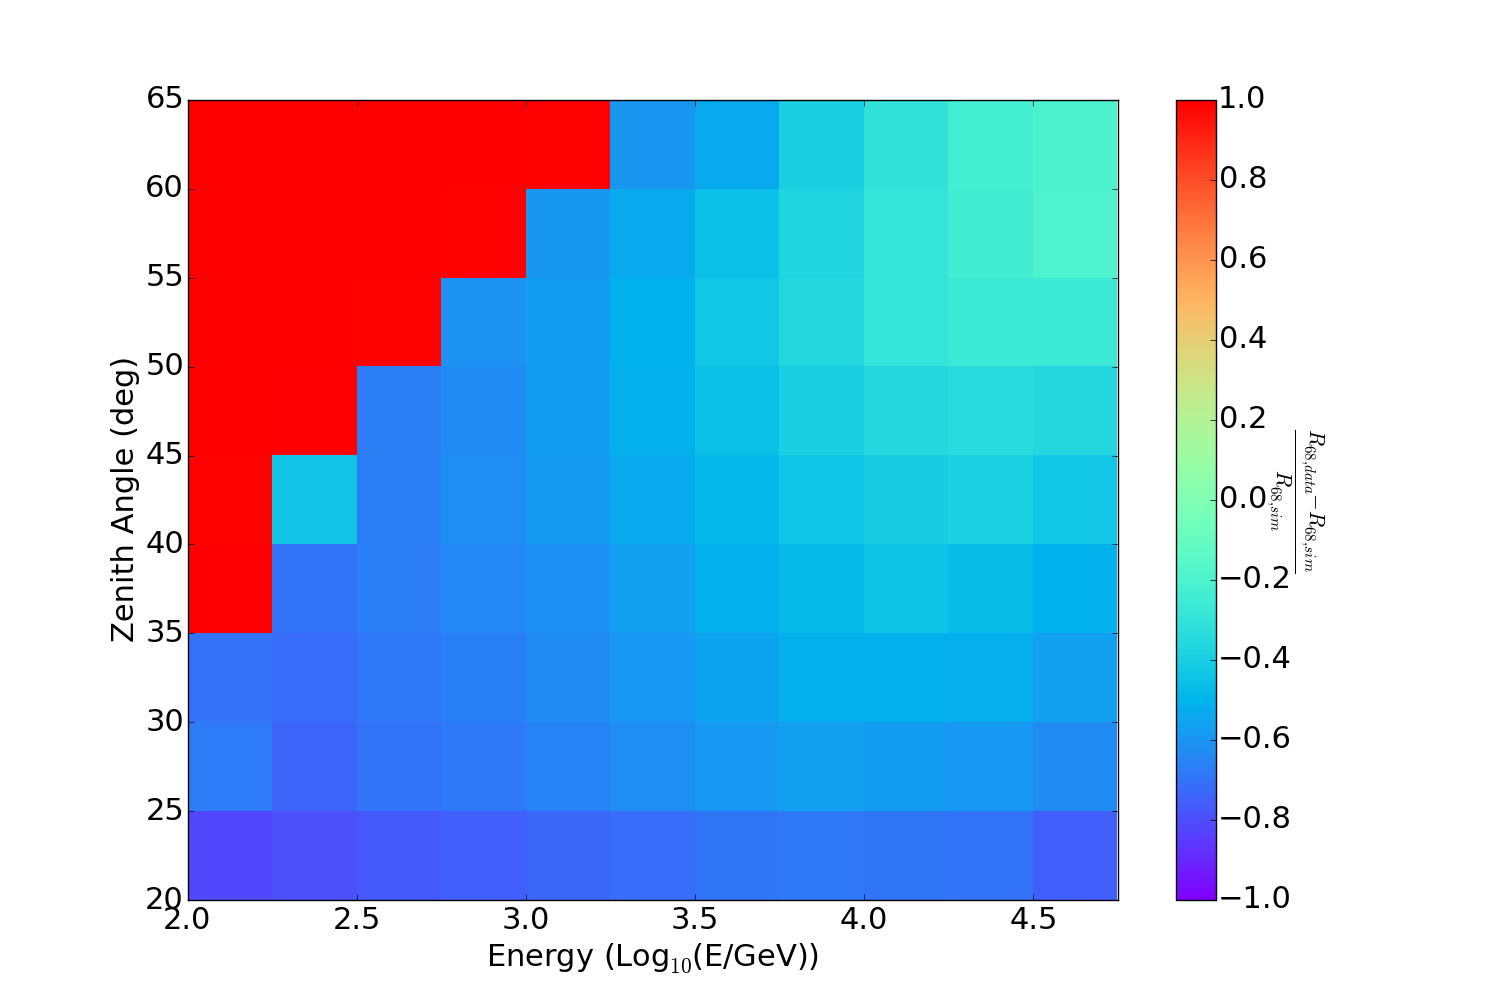
\includegraphics[width=0.47\linewidth]{num/LZA_data_25/crab_disp_sim.png}
      \label{fig:crab_disp_sim}
    }
    \subfigure[Number of excess events ($\log(N_{on}-\alpha N_{off})$).]{ 
      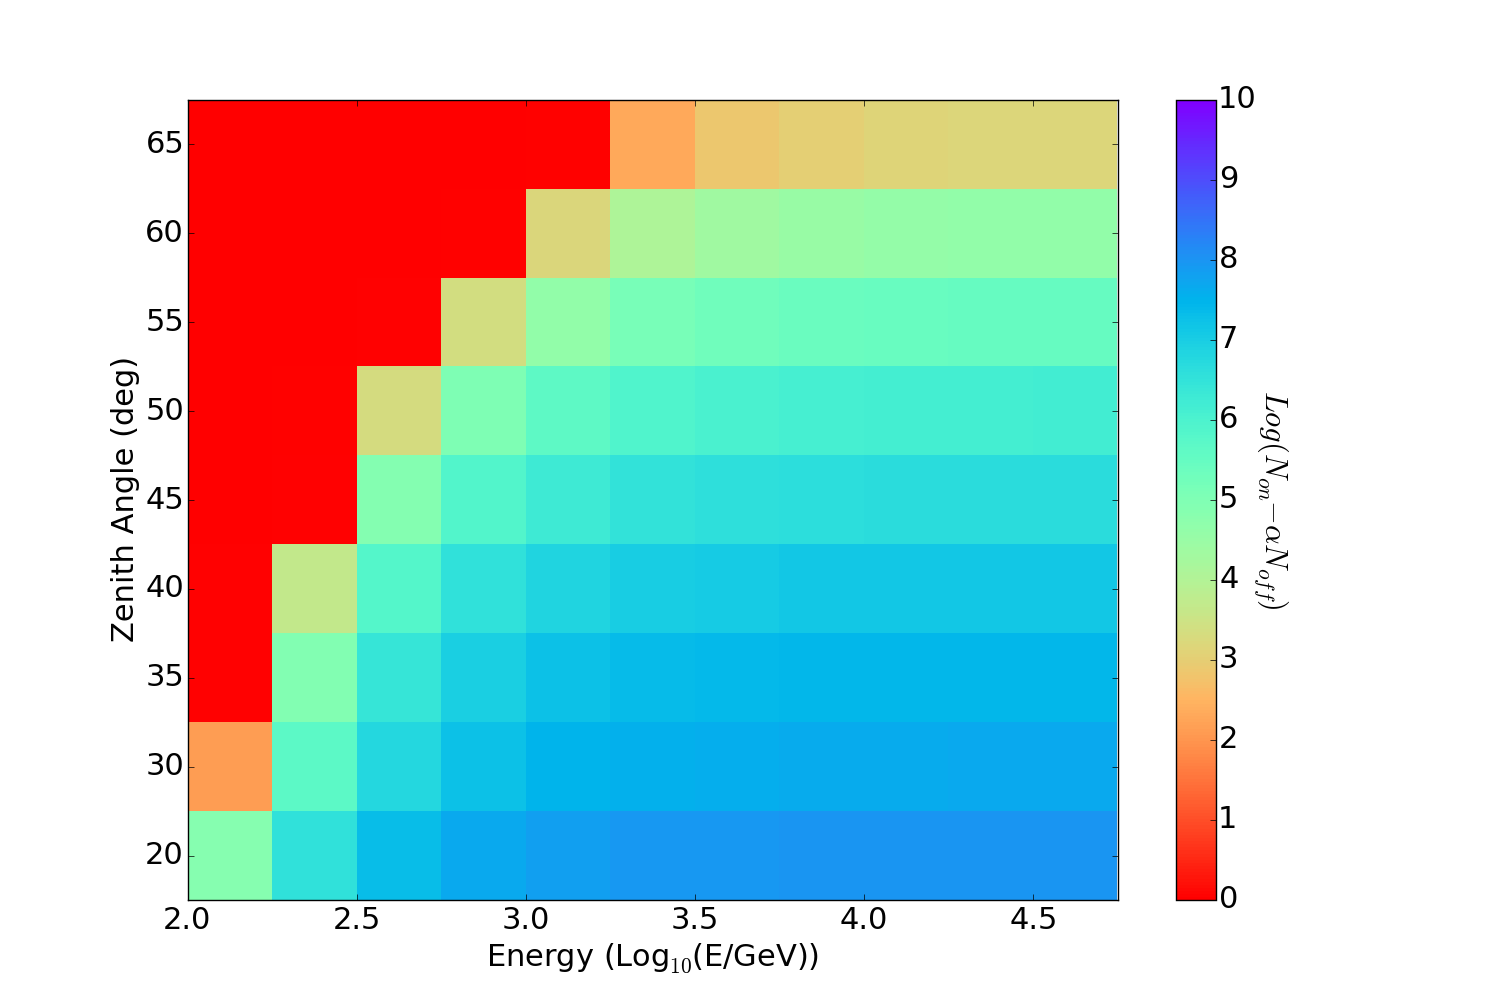
\includegraphics[width=0.47\linewidth]{num/LZA_data_25/crab_disp_Log_nevent.png}
      \label{fig:crab_disp_nevent}
    }  
    \subfigure[Li \& Ma significance.]{ 
      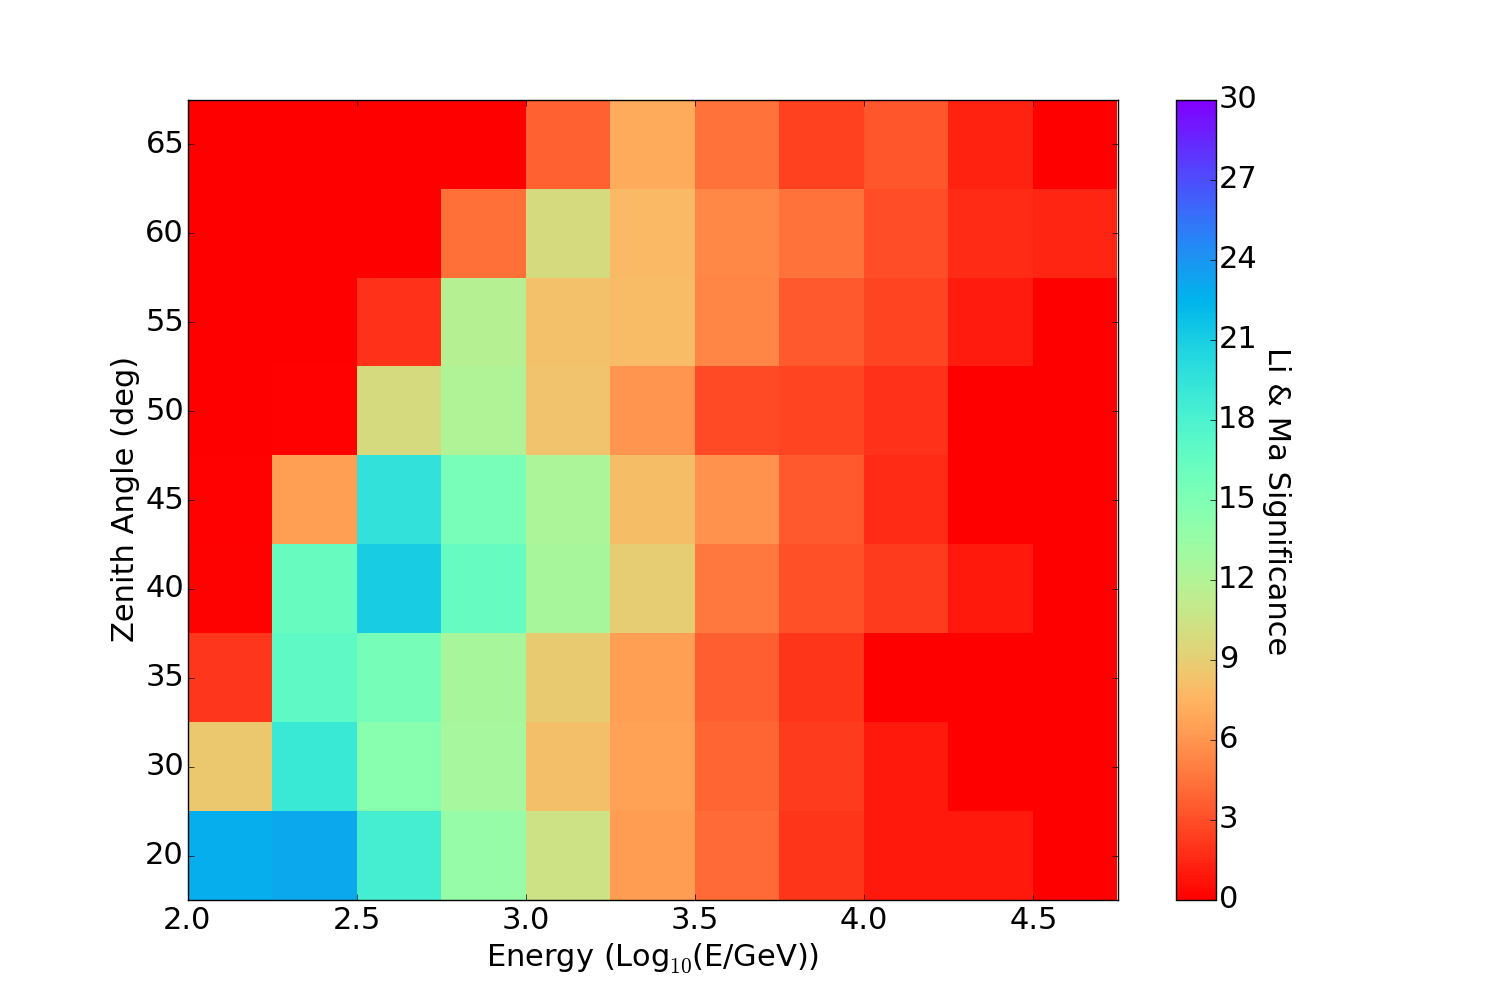
\includegraphics[width=0.47\linewidth]{num/LZA_data_25/crab_disp_LiMa.png}
      \label{fig:crab_disp_li_ma}
    }
  \end{center}
  \caption[Crab (horizon-to-horizon runs) direction reconstruction using Method5t.]{Reconstruction of the direction of the Crab Nebula horizon-to-horizon runs using the new \disp tables. In the top two plots, white denotes regions of significance $<3\sigma$. Relative to Fig. \ref{fig:crab_initial}, this provides better resolution at the highest zenith angles, and is able to reconstruct higher-energy events in the $45-55^\circ$ region.}
  \label{fig:crab_disp}
\end{figure}
Relative to Fig. \ref{fig:crab_initial}, this provides better resolution at the highest zenith angles and is able to reconstruct higher-energy events in the $45-55^\circ$ region. This provides a proof-of-principle that the \disp method is an improvement on the standard method at the highest energies and at the large zenith angles. In the region $\phi\geq50$ and $E\geq 1$ TeV the Crab nebula has a \rse of $\sim 0.15^\circ$.
\begin{figure}[H]
  \begin{center}
    \subfigure[Angular resolution using Method5t.]{ 
      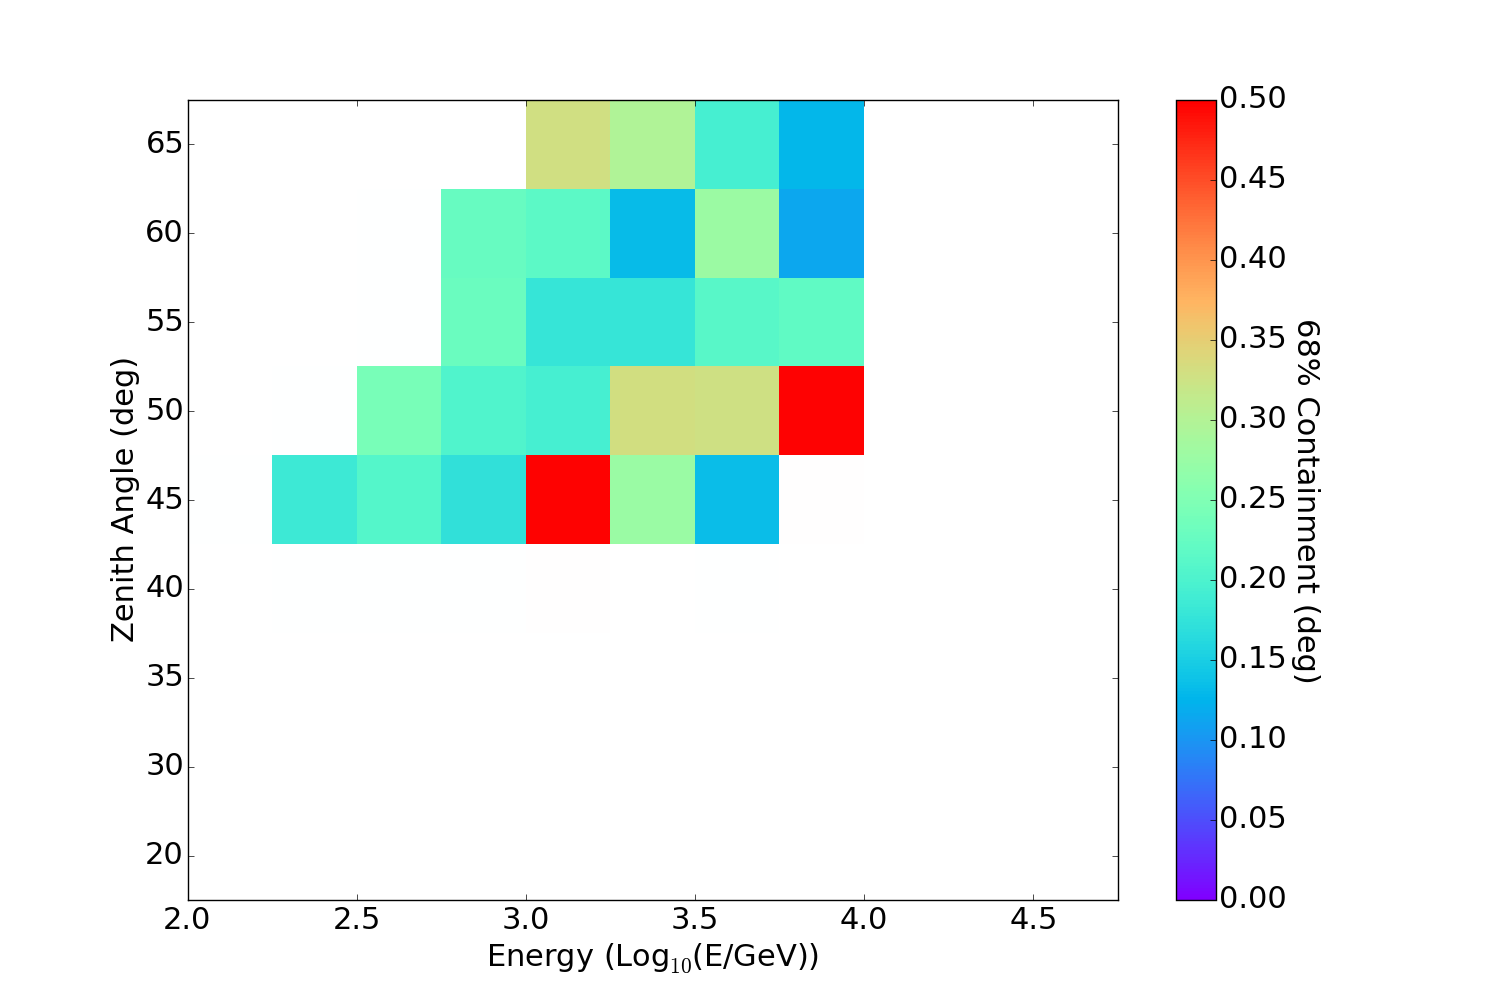
\includegraphics[width=0.47\linewidth]{num/LZA_data_25/crab_all_disp_rse.png}
      \label{fig:crab_all_disp_rse}
    }  
    \subfigure[Deviation from simulations ($\xi$).]{ 
      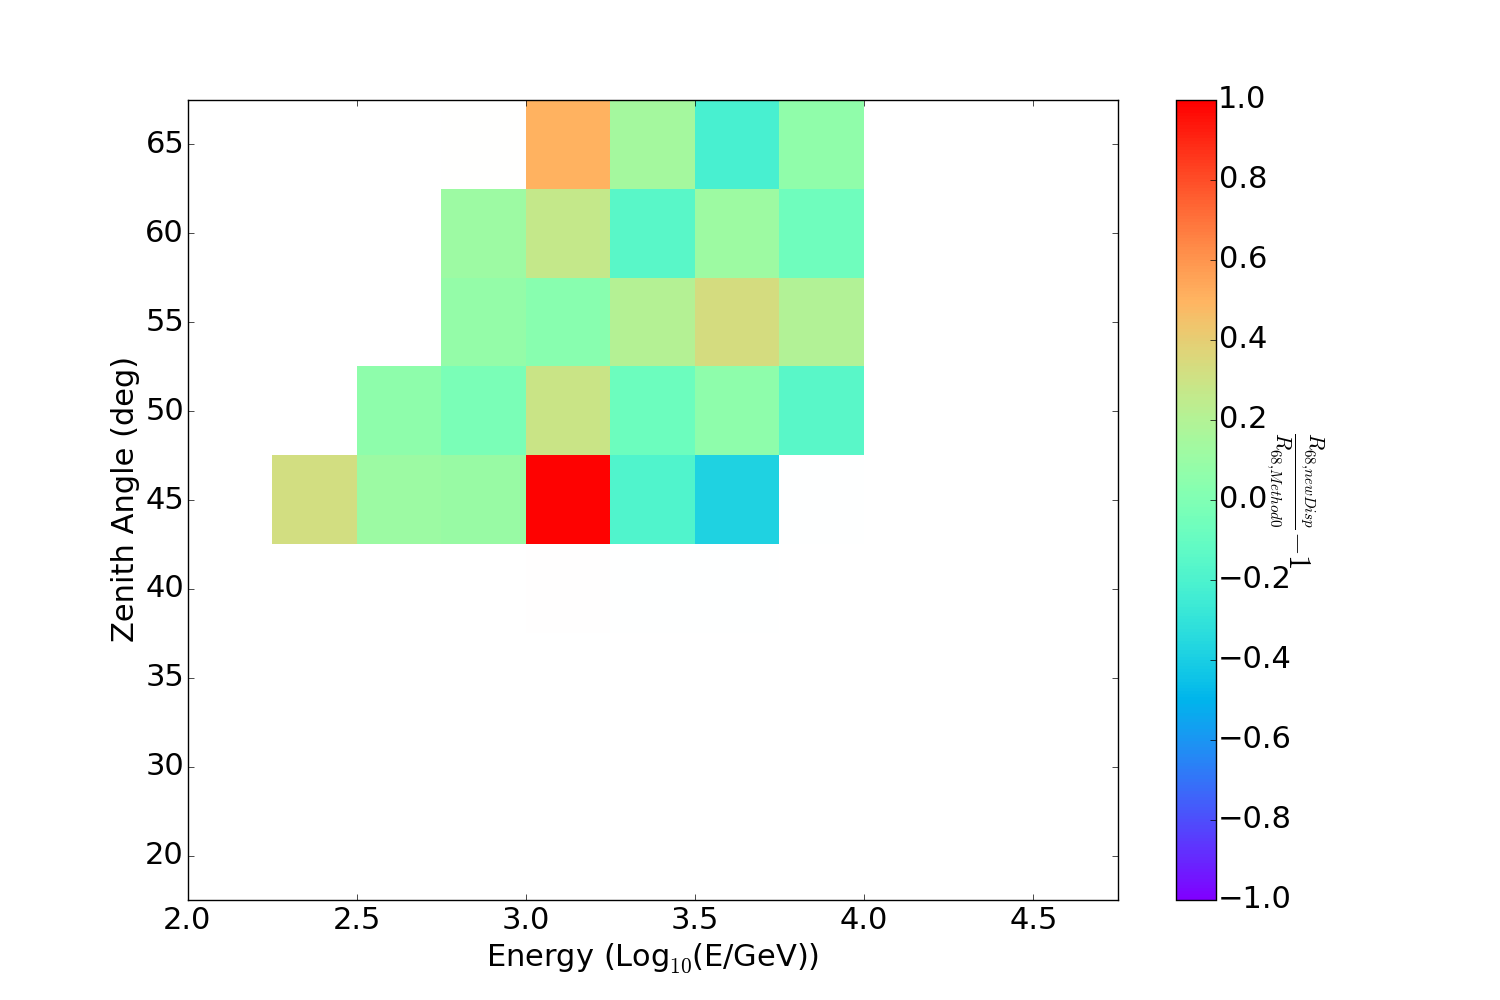
\includegraphics[width=0.47\linewidth]{num/LZA_data_25/crab_all_disp_sim.png}
      \label{fig:crab_all_disp_sim}
    }
    \subfigure[Number of excess events ($\log(N_{on}-\alpha N_{off})$).]{ 
      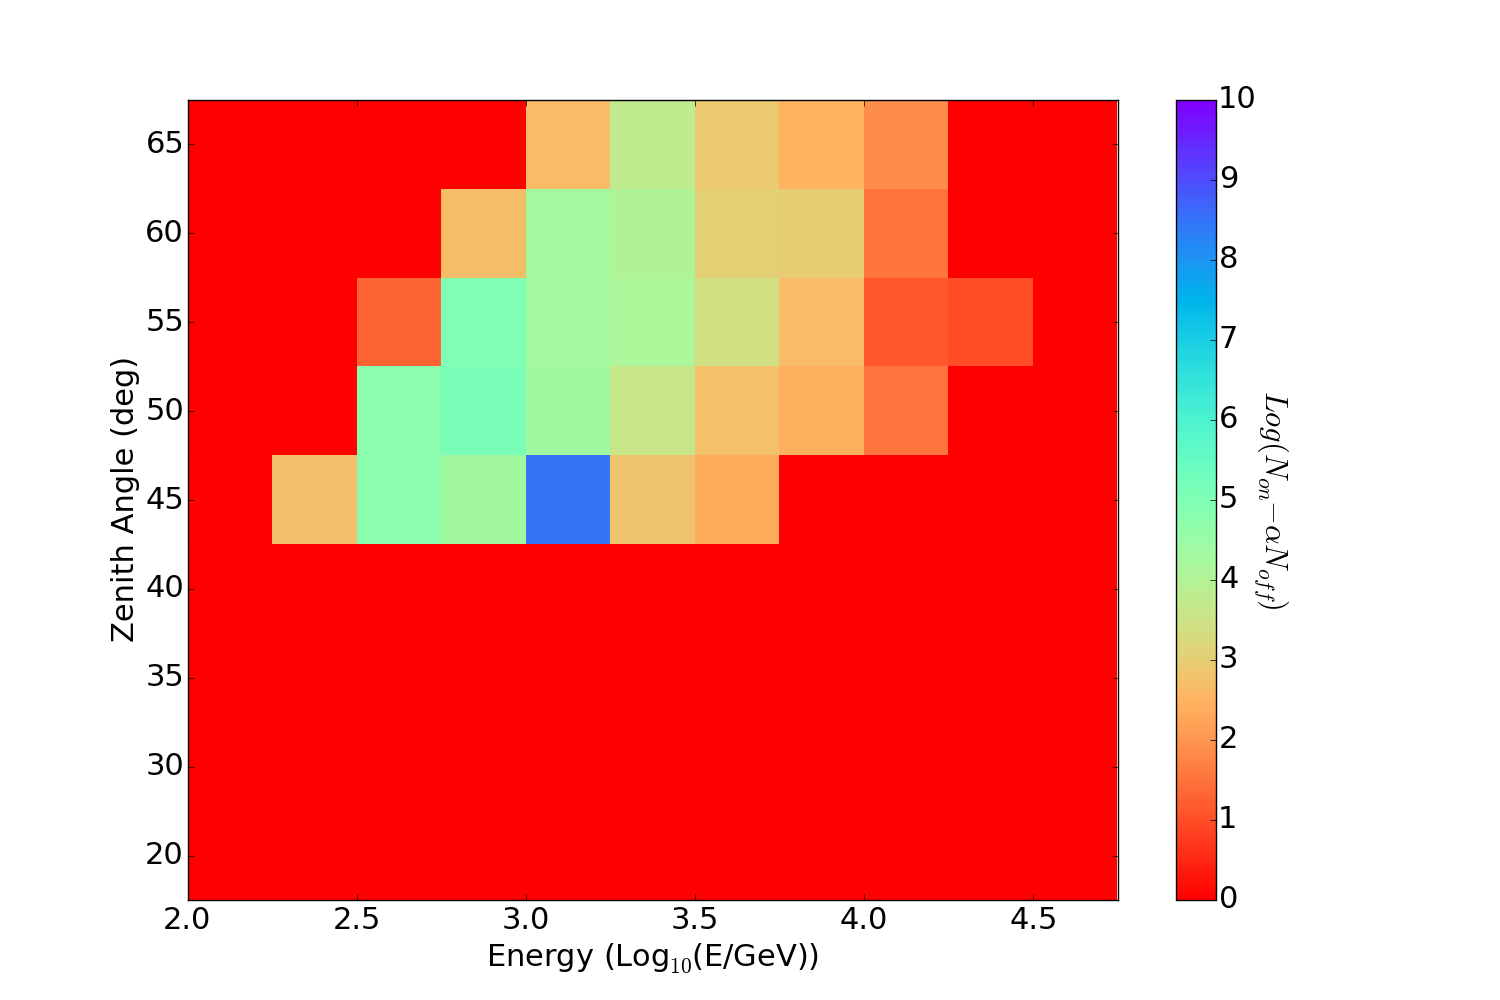
\includegraphics[width=0.47\linewidth]{num/LZA_data_25/crab_all_disp_Log_nevent.png}
      \label{fig:crab_all_disp_nevent}
    }  
    \subfigure[Li \& Ma significance.]{ 
      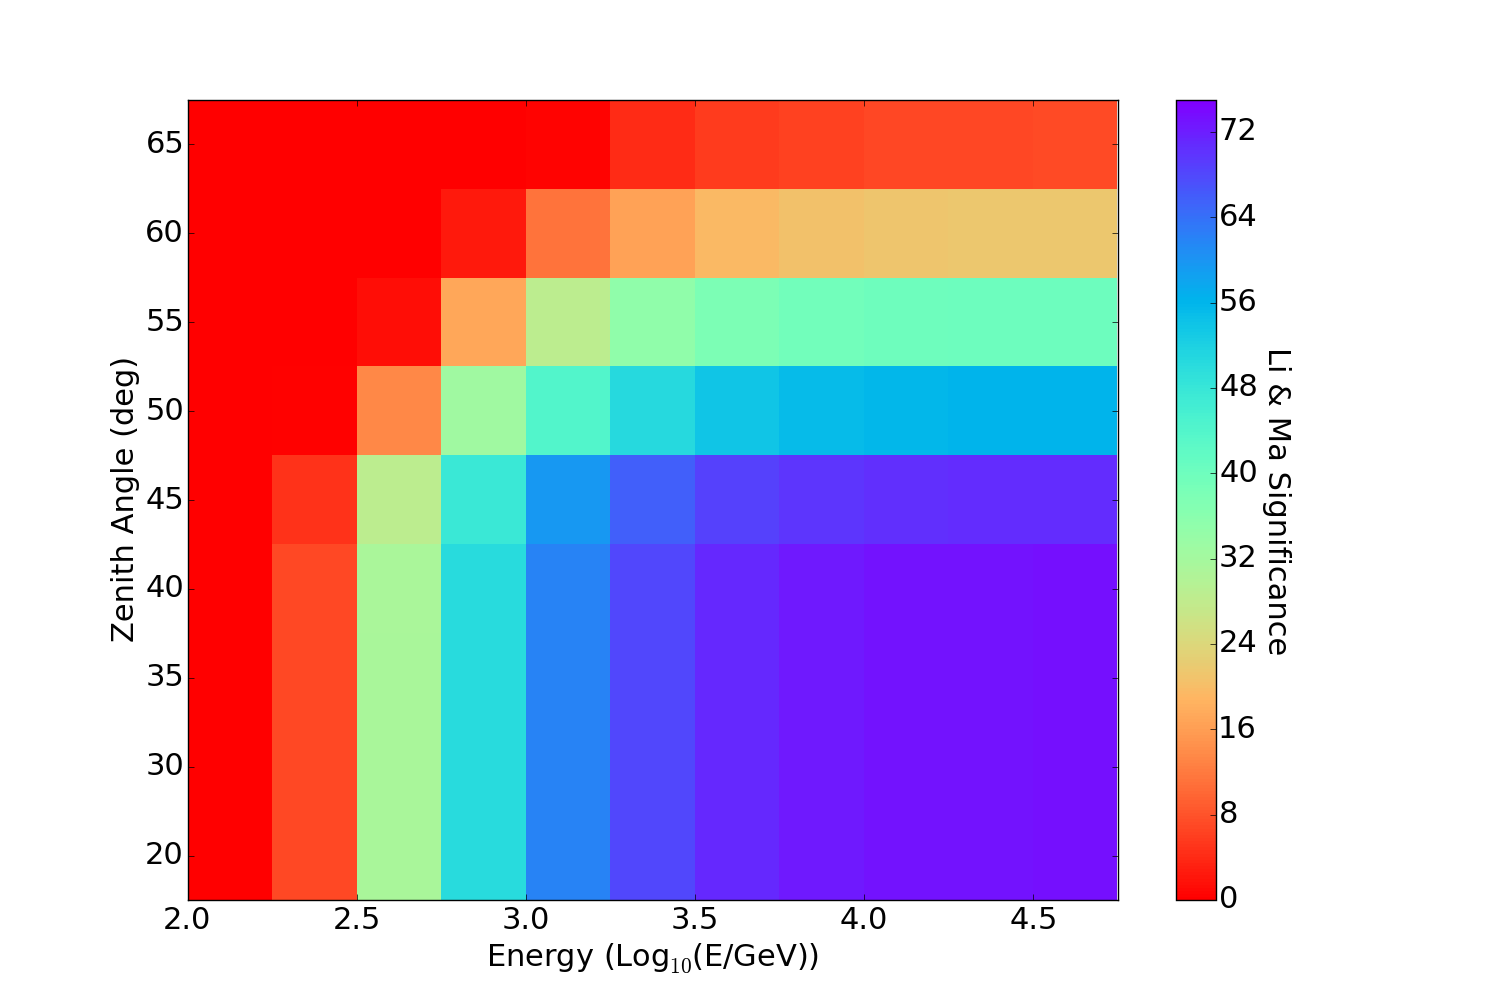
\includegraphics[width=0.47\linewidth]{num/LZA_data_25/crab_all_disp_LiMa.png}
      \label{fig:crab_all_disp_li_ma}
    }
  \end{center}
  \caption[Crab (LZA runs) direction reconstruction using Method5t.]{Reconstruction of the direction of the Crab Nebula LZA runs using the new \disp tables. In the top two plots, white denotes regions of significance $<3\sigma$.}
  \label{fig:crab_all_disp}
\end{figure}

The numbers for the Crab Nebula in Fig. \ref{fig:crab_disp} suggest that we can not yet detect the extension of the Crab, which is consistent with the simulation analysis. Also expected from the simulation results, the \rse decreases with increasing energy. In the regime of interest, ($E>1$ TeV and $\phi\gtrsim 50^\circ$), the data reconstruction under-performs relative to simulations with $\xi\sim 0.3$, and the dependence of the \rse (see Fig. \ref{fig:crab_all_disp_rse}) on zenith angle is smaller than expected. This is perhaps due to lower statistics in the region (see Fig. \ref{fig:crab_all_disp_nevent}), since for most of our parameter space, $|\xi| \leq 0.15$ (Fig. \ref{fig:crab_all_disp_sim}).

\subsection{\rse for Mrk421}
Mrk421 is an extra-galactic source ($z=0.031$) with a hard spectrum (spectral index $\Gamma=2.2$), but less than 5 hours of observation in the zenith range of interest ($\phi>45^\circ$). Even with a short total duration of observation, because Mrk421 is a high-flux object, it is still observable at high significance. In the region $\phi\geq50$ and $E\geq 1$ TeV Mrk 421 has a \rse of $\sim 0.11^\circ$.

The result of this analysis was that the smallest values of \rse for Mrk421 ($\sim 0.09^\circ$, Fig. \ref{fig:mrk_rse}) are found in a region of parameter space where the Li \& Ma significance is small (Fig. \ref{fig:mrk_li_ma}) and more generally that the high values of $\xi$ are found where Li \& Ma significance is low, suggesting that a more robust analysis would require more statistics. Consequently this point-source analysis does not definitively validate the results from the simulations but it does demonstrate the simulation result that the point-source reconstruction in the regime of interest is $<0.2^\circ$ (Fig. \ref{fig:mrk_rse}).

\begin{figure}[H]
  \begin{center}
    \subfigure[Angular resolution using Method5t.]{ 
      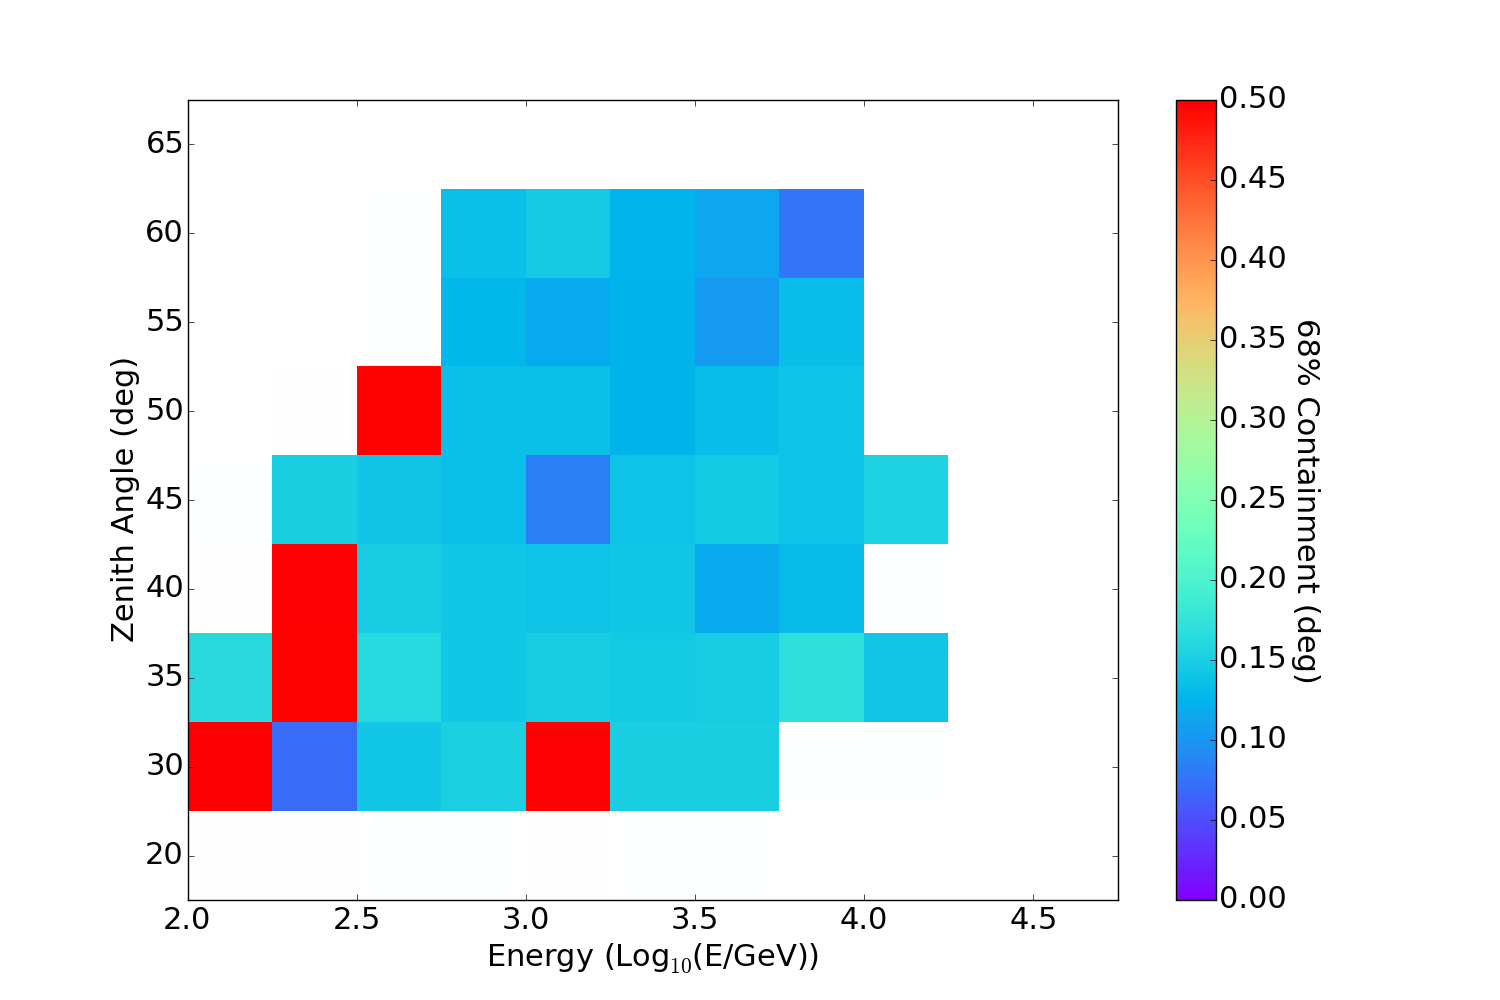
\includegraphics[width=0.47\linewidth]{num/LZA_data_25/Mrk421_rse.png}
      \label{fig:mrk_rse}
    }  
    \subfigure[Deviation from simulations ($\xi$).]{ 
      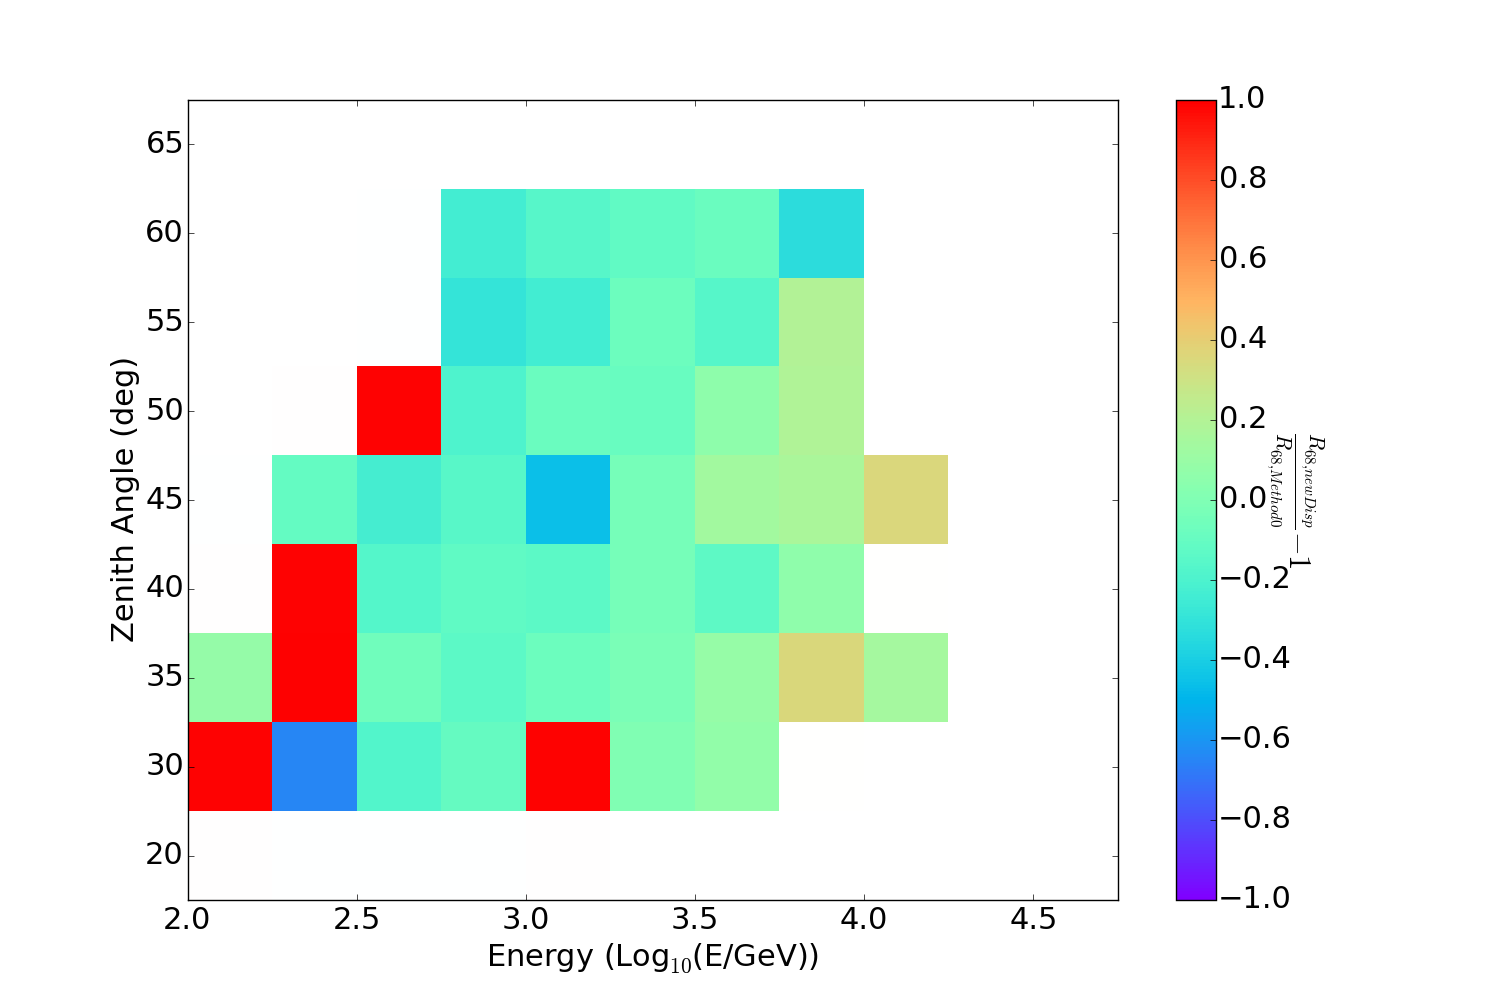
\includegraphics[width=0.47\linewidth]{num/LZA_data_25/Mrk421_sim.png}
      \label{fig:mrk_sim}
    }
    \subfigure[Number of excess events ($\log(N_{on}-\alpha N_{off})$).]{ 
      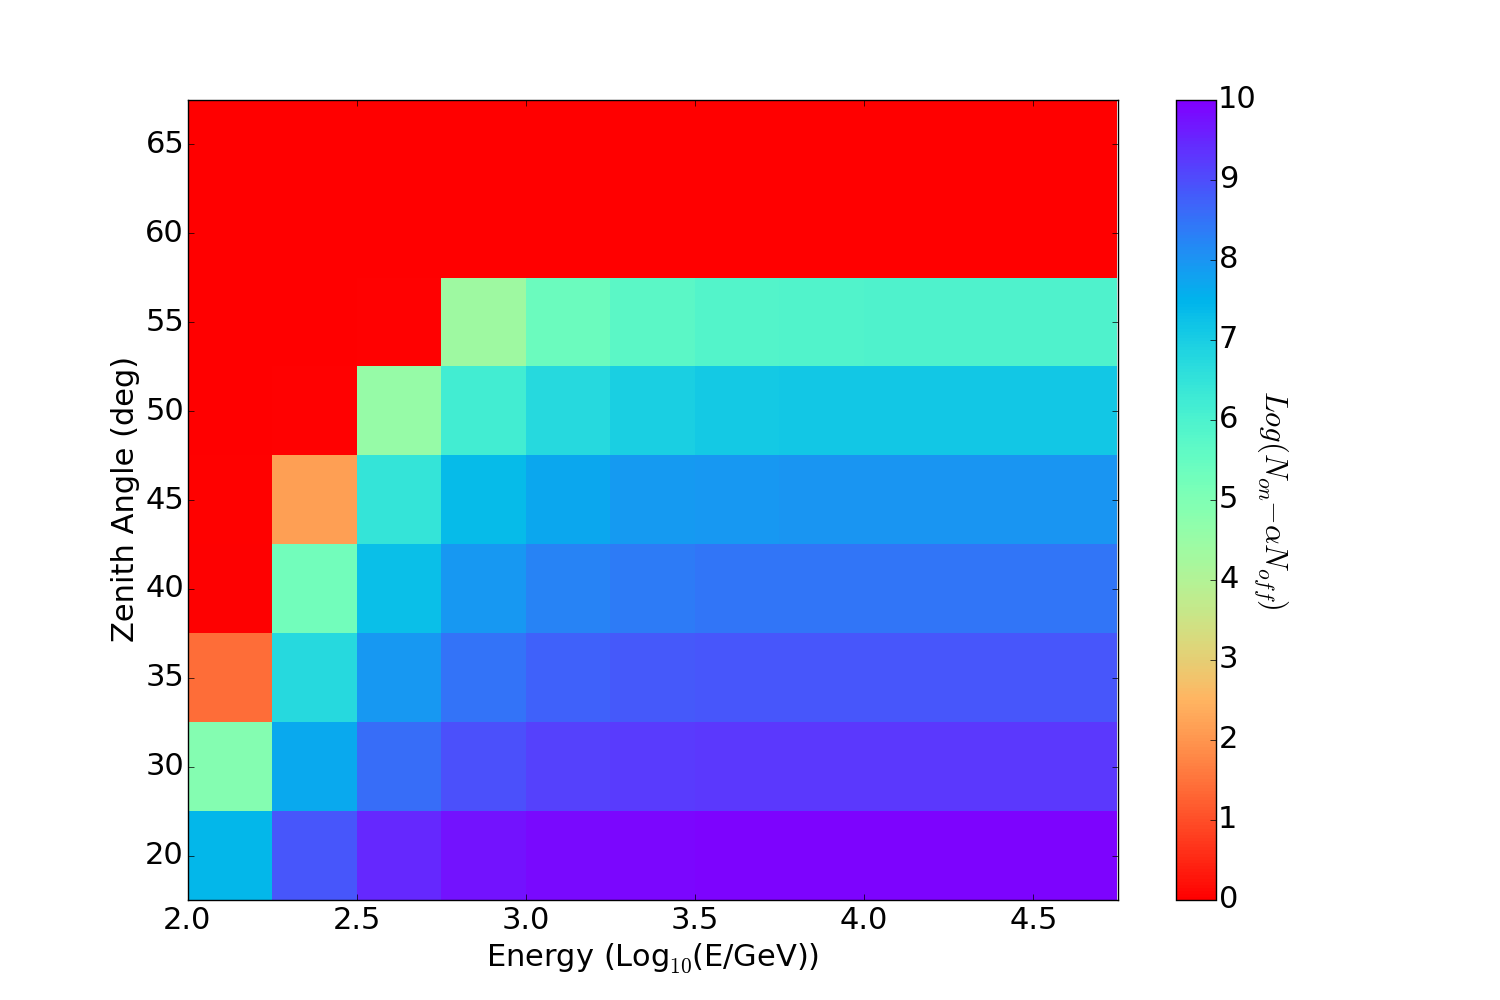
\includegraphics[width=0.47\linewidth]{num/LZA_data_25/Mrk421_Log_nevent.png}
      \label{fig:mrk_nevent}
    }  
    \subfigure[Li \& Ma significance.]{ 
      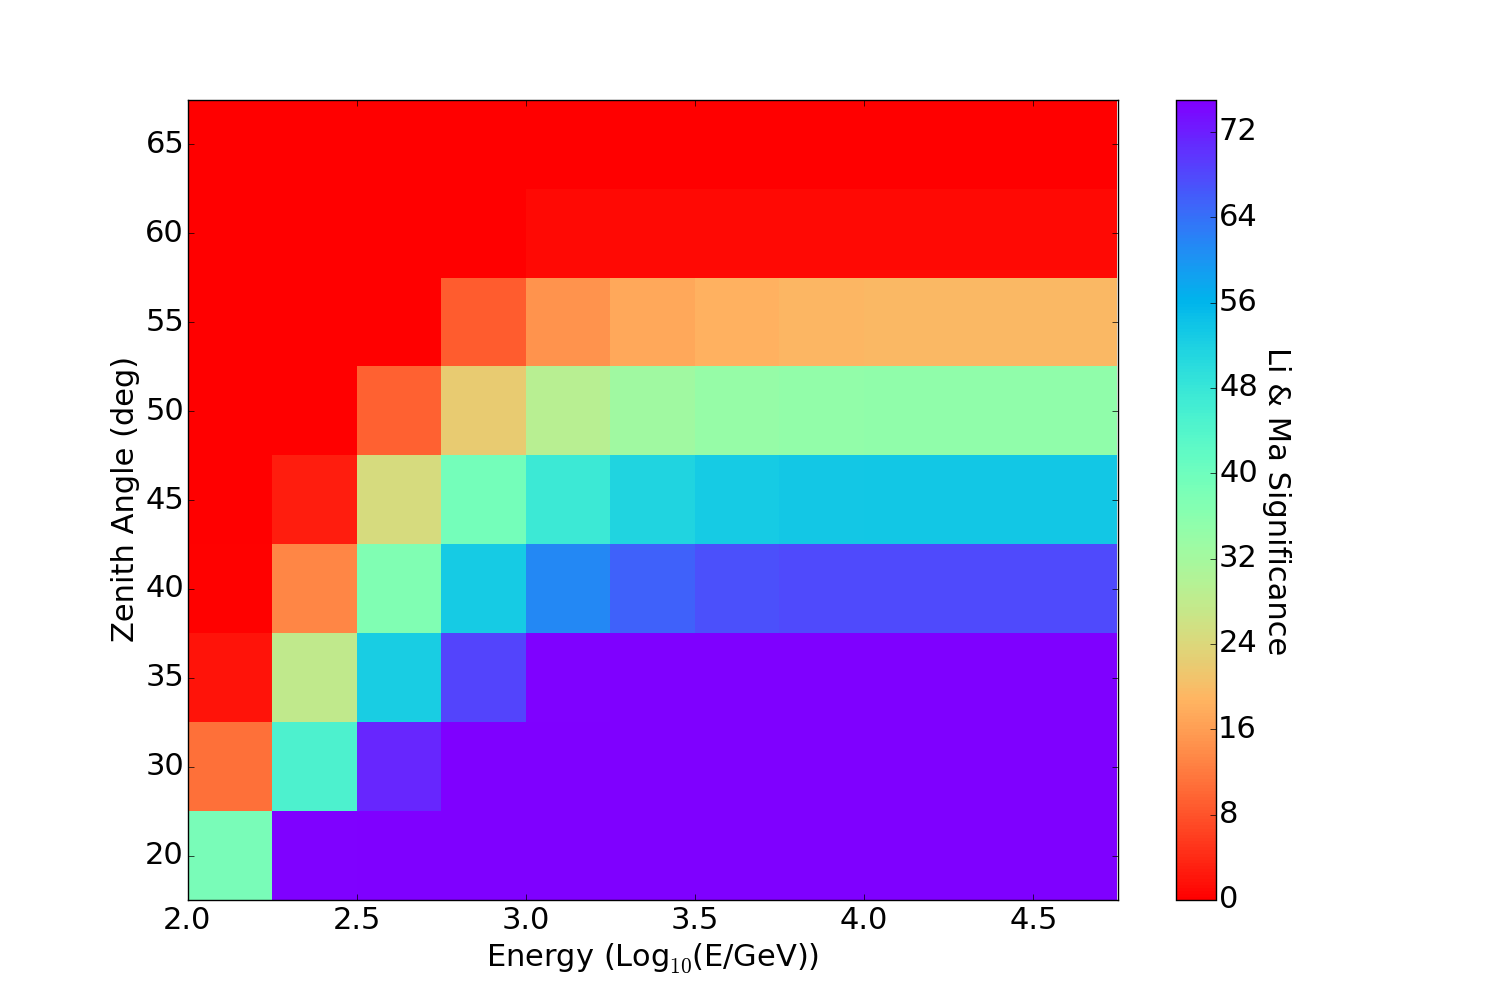
\includegraphics[width=0.47\linewidth]{num/LZA_data_25/Mrk421_LiMa.png}
      \label{fig:mrk_li_ma}
    }
  \end{center}
  \caption[Mrk421 direction reconstruction using Method5t.]{Reconstruction of the direction of Mrk421 using the new \disp tables. In the top two plots, white denotes regions of significance $<3\sigma$.}
  \label{fig:mrk_disp}
\end{figure}

% \subsection{\rse for PKS1510-089}
% PKS1510-089 is an extra-galactic source ($z=0.361$) with a softer spectrum (spectral index $\Gamma=3.26$), but 17 hours of observation in the zenith range of interest ($\phi>40$). Analysis of the data reveals that none of this falls in the region of best performance ($\phi>45$ and $E>10$TeV)

% \begin{figure}[H]
%   \begin{center}
%     \subfigure[Angular resolution using Method5t.]{ 
%       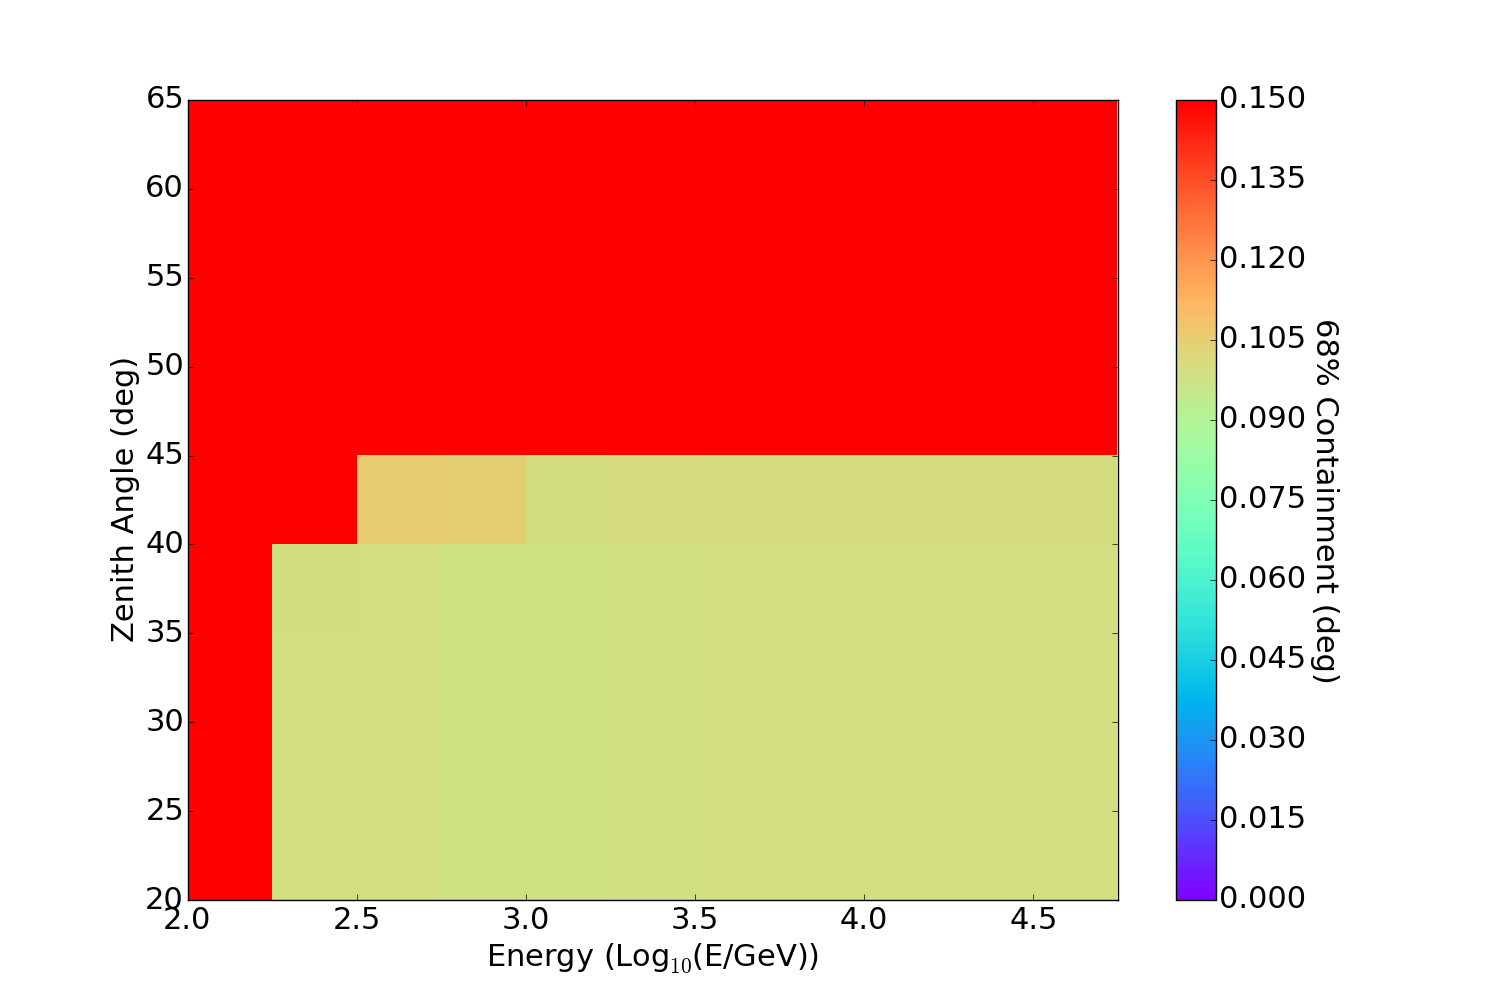
\includegraphics[width=0.47\linewidth]{PKS1510_rse.png}
%       \label{fig:PKS1510_rse}
%     }  
%     \subfigure[Deviation from simulations ($\xi$).]{ 
%       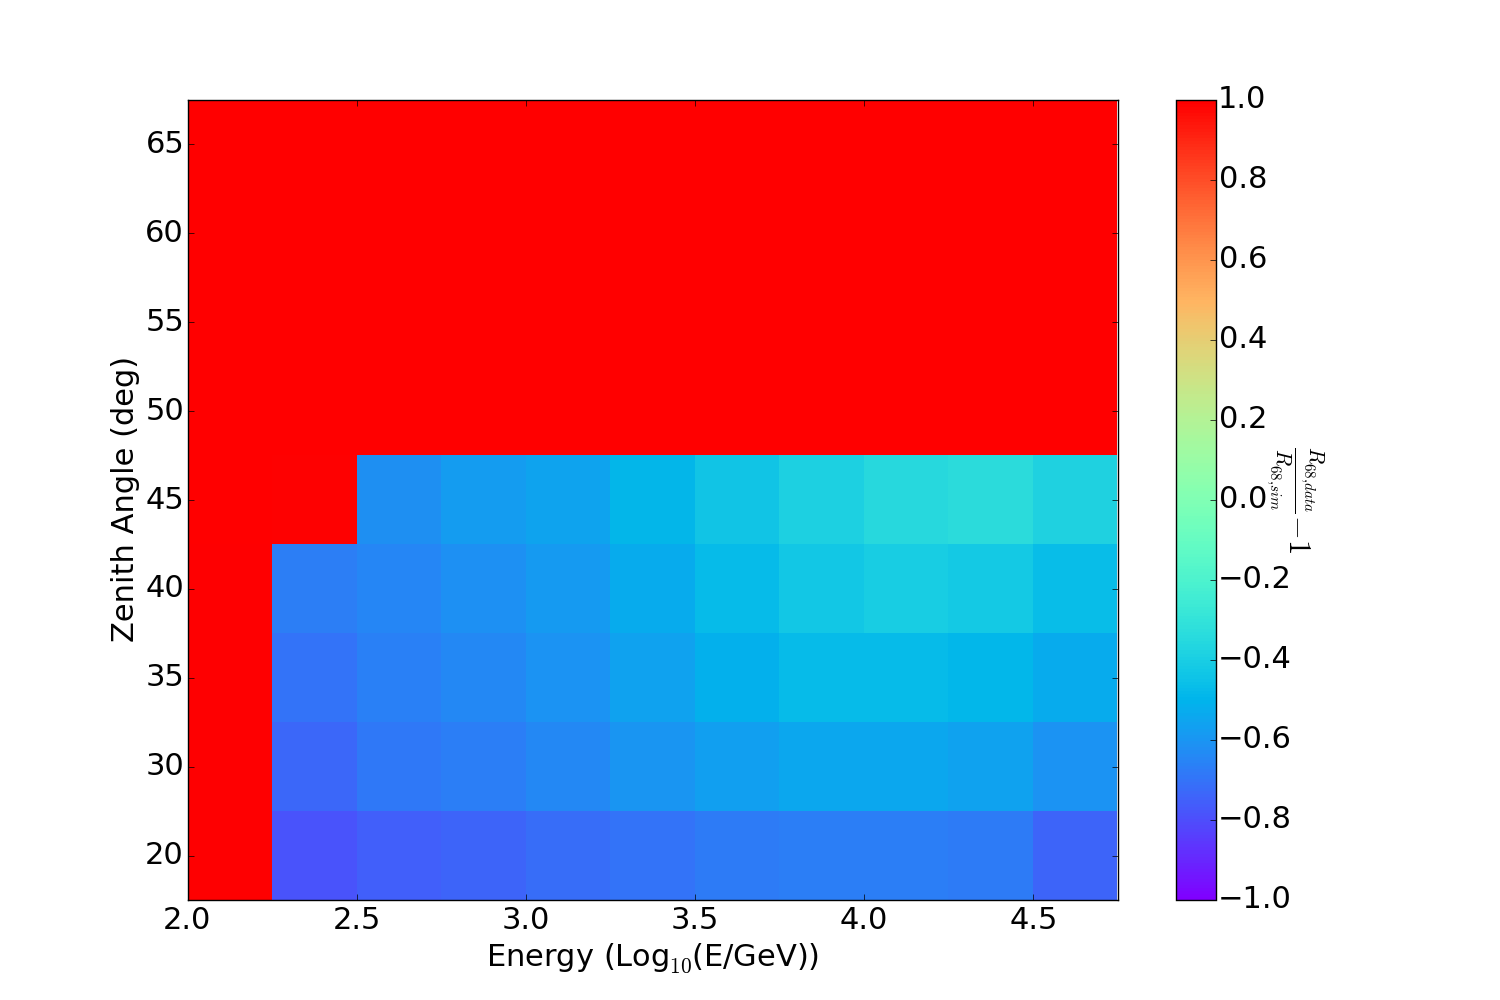
\includegraphics[width=0.47\linewidth]{PKS1510_sim.png}
%       \label{fig:PKS1510_sim}
%     }
%     \subfigure[Number of excess events ($\log(N_{on}-\alpha N_{off})$).]{ 
%       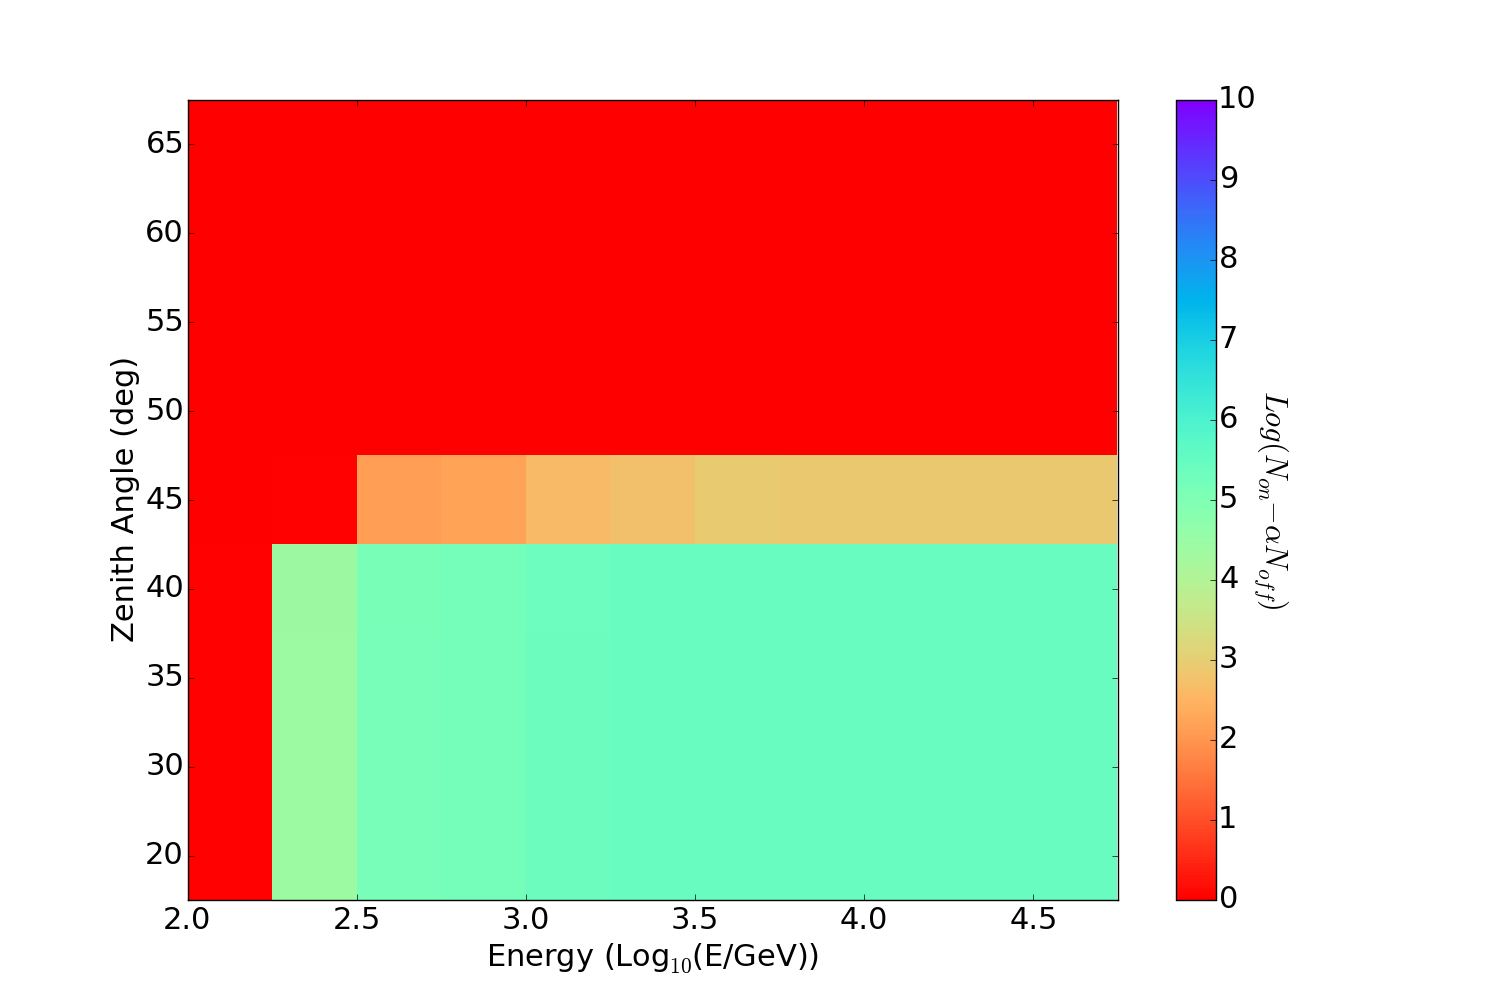
\includegraphics[width=0.47\linewidth]{PKS1510_Log_nevent.png}
%       \label{fig:PKS1510_nevent}
%     }  
%     \subfigure[Li \& Ma significance.]{ 
%       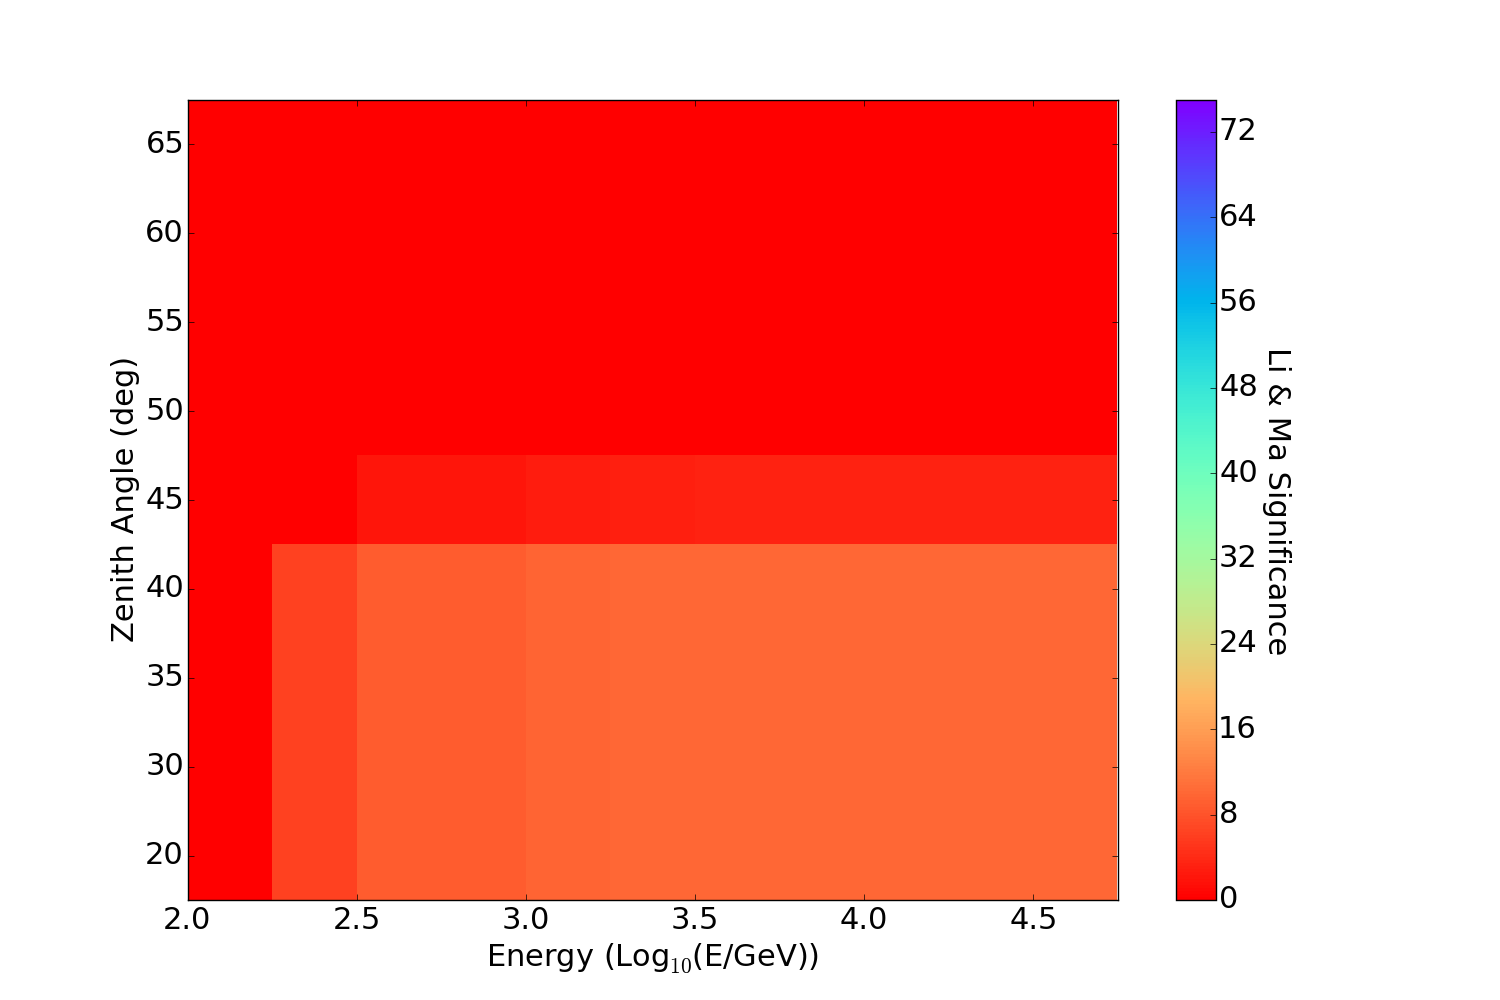
\includegraphics[width=0.47\linewidth]{PKS1510_LiMa.png}
%       \label{fig:PKS1510_li_ma}
%     }
%   \end{center}
%   \caption[PKS1510 direction reconstruction using Method5t.]{Reconstruction of the direction of PKS1510 using the new \disp tables.  In each case red denotes regions of no statistics.}
%   \label{fig:PKS1510_disp}
% \end{figure}

\end{document}
